\section{Introducción al análisis numérico con Abaqus}

\subsection{Motivación}

\paragraph{Introducción al programa Abaqus.} Abaqus es un programa (o
un conjunto de programas) para realizar análisis por elementos finitos
en el que hay dos formas de trabajar:
\begin{enumerate}
\item \textbf{Interactive:} Usando la interfaz gráfica de usuario
  Abaqus/CAE (Fig.~\ref{figu10}).
  \begin{itemize}
  \item No es necesario aprender la sintaxis del fichero de entrada del programa.
  \item Más costoso cambiar un parámetro y realizar de nuevo el
    análisis.
  \end{itemize}
  \begin{figure}
    \begin{center}
      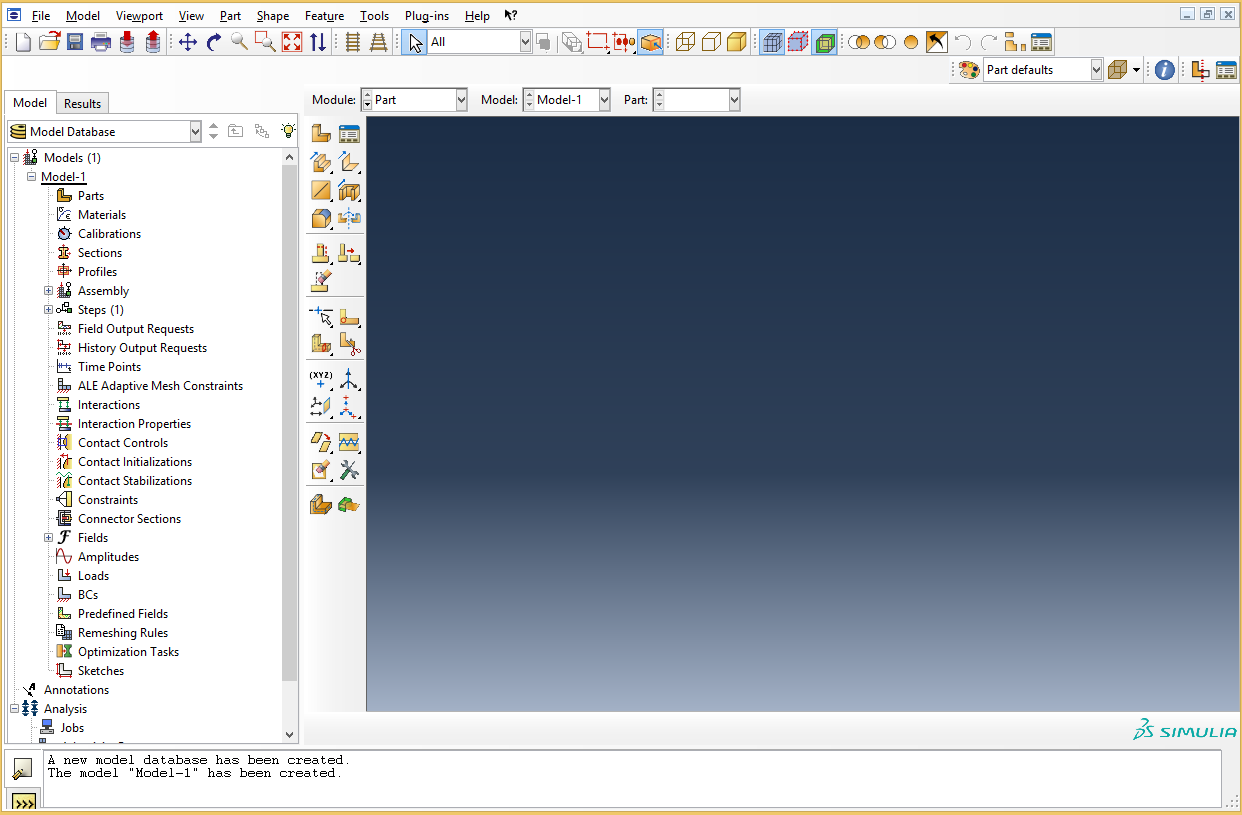
\includegraphics[width=0.9\textwidth]{./body/images/imagen10}
    \end{center}
    \caption{Interfaz gráfica Abaqus/CAE}
    \label{figu10}
  \end{figure}
\item \textbf{Keywords:} Se construye un fichero de entrada
  \texttt{.inp} tipo texto plano con los comandos necesarios para
  realizar el análisis (Fig.~\ref{figu09}).
  \begin{itemize}
  \item Hay que saberse la sintaxis del fichero de entrada  del programa.
  \item Es muy fácil modificar algo y realizar un nuevo análisis
  \item Aunque trabajemos en modo \textit{interactive}, al final
    Abaqus siempre genera un fichero de texto plano.
  \end{itemize}
  \begin{figure}[H]
    \begin{center}
      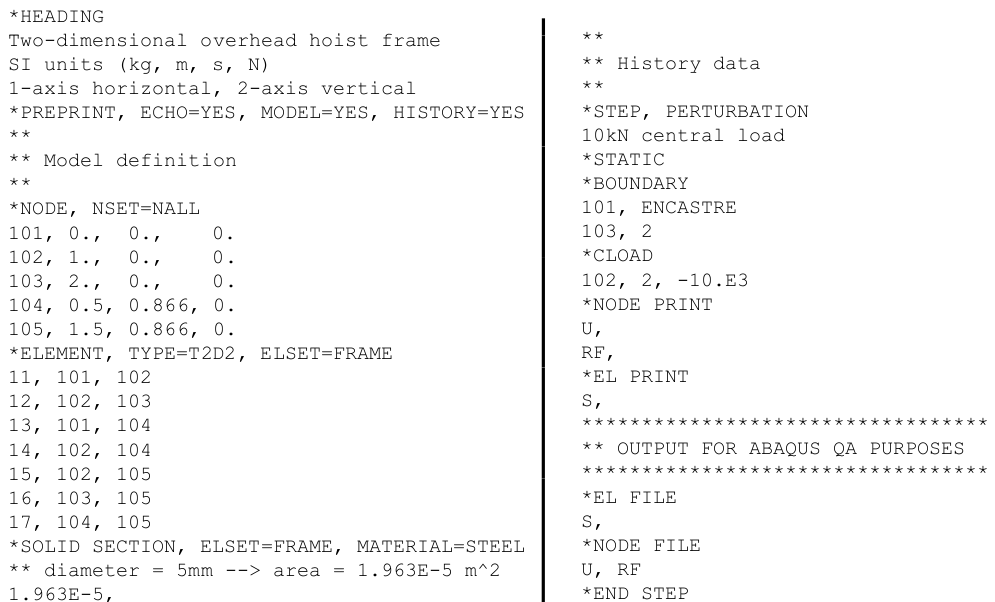
\includegraphics[width=0.8\textwidth]{./body/images/imagen09}
    \end{center}
    \caption{Ejemplo fichero .inp}
    \label{figu09}
  \end{figure}
\end{enumerate}

Nosotros vamos a trabajar en modo \textit{interactive}. Para arrancar
el programa de preproceso gráfico Abaqus/CAE debemos escribir
\textbf{abaqus cae} en la consola de comandos o pulsar el enlace
directo. Una vez arrancado, de las opciones que nos da elegiremos
\textbf{Create Model Database with Standard/Explicit Model} tal como
indica la Fig.~\ref{figu00})
\begin{figure}
  \begin{center}
    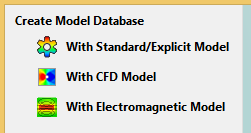
\includegraphics[width=0.4\textwidth]{./body/images/imagen00}
  \end{center}
  \caption{Inicio programa Abaqus}
  \label{figu00}
\end{figure}

Nos aparece el entorno de trabajo de Abaqus/CAE donde podemos
identificar las siguientes secciones (Fig.~\ref{figu11}):
\begin{itemize}
\item \textit{Viewport:} Parte principal de la pantalla de Abaqus/CAE
  donde visualizamos el pre y postproceso de nuestro análisis.
\item \textit{Model Tree View:} Todos los pasos que seguimos en
  nuestro modelo se representan en esta sección en forma de nodos del
  árbol. Cada nodo se subdivide en varios subnodos con sus
  funcionalidades correspondientes. Si el \textit{Model Tree} no está
  visible, hazlo visible pulsando \textbf{View/Show Model Tree} o
  pulsando \texttt{CTRL+T}.
\item \textit{Toolbar Section:} A cada nodo del \textit{Model Tree} le
  corresponde una barra de herramientas donde el usuario puede acceder
  a los comandos asociados. Podemos acceder a estos comandos también
  mediante los menús desplegables de la barra superior (aunque en este
  tutorial usaremos los iconos gráficos de la barra de herramientas).
\item \textit{Prompt region:} Cuando seleccionamos un cierto comando,
  en la región \textit{Prompt} aparece información sobre la siguiente
  acción a realizar.
\end{itemize}

\begin{figure}[H]
  \begin{center}
    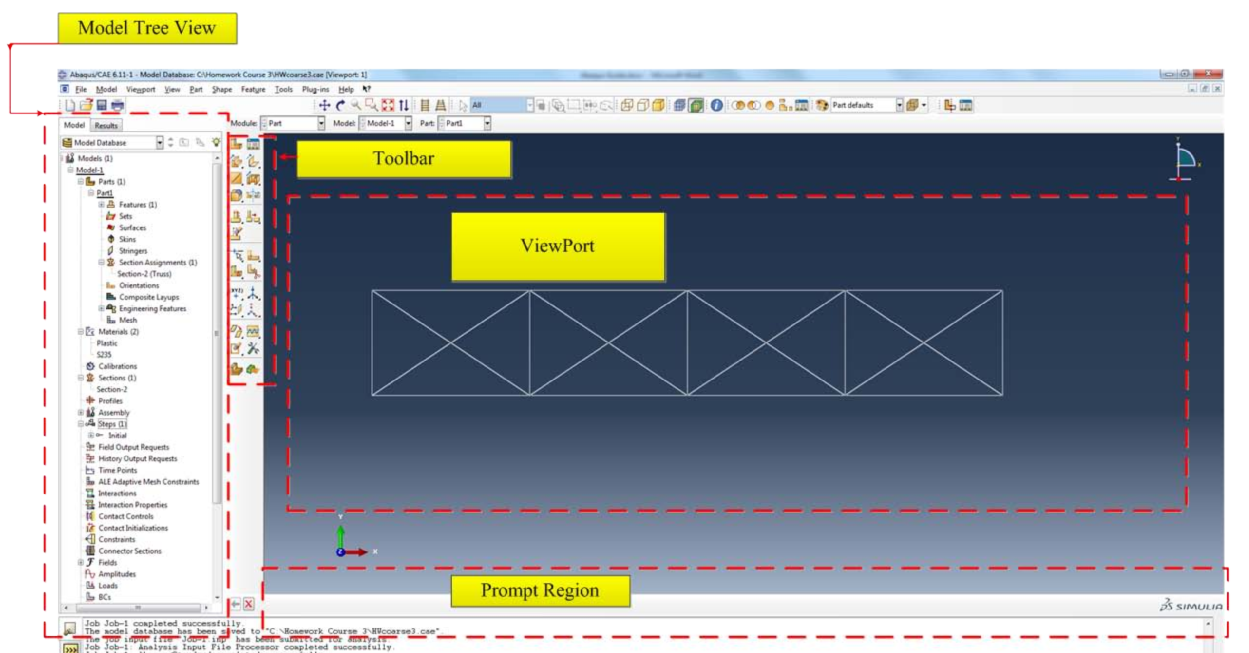
\includegraphics[width=1.05\textwidth]{./body/images/imagen11}
  \end{center}
  \caption{Descripción espacio de trabajo Abaqus CAE}
  \label{figu11}
\end{figure}




\paragraph{Fases del análisis} Para realizar un análisis de elementos
finitos debemos realizar una serie de pasos. Abaqus ha agrupado estos
pasos en \textbf{Módulos} secuenciales. A continuación se resumen los
funcionalidades asociadas a cada módulo\footnote{Los módulos con
  asterisco * no los vamos a usar en este curso}:
\begin{description}
\item[Módulo Part.] Crear la geometría de los elementos.
  (\textit{Parts})
  \begin{enumerate}
  \item Bosquejar los elementos de la geometría del dominio
  \item Crear \textit{Parts} con los elementos de la geometría del
    dominio
  \end{enumerate}
\item[Módulo Property.] Definir materiales y secciones.
  \begin{enumerate}
  \item Definir las propiedades de los materiales
  \item Definir las secciones (que asociamos a los materiales)
  \item Asignar las secciones a las \textit{Parts} correspondientes.
  \end{enumerate}
\item[Módulo Assembly.] Ensamblar el modelo creando copias
  (instancias) de las \textit{Parts}.
\item[Módulo Step.] Configurar el procedimiento de análisis.
  \begin{enumerate}
  \item Definir los pasos de cálculo
  \item Definir el tipo de análisis en cada paso de cálculo (térmico,
    mecánico, estacionario, transitorio,\ldots)
  \item Definir las variables que el programa debe guardar para
    visualizar en el postproceso
  \item Definir los parámetros de los algoritmos numéricos utilizados
    en cada paso de cálculo.
  \end{enumerate}
\item[Módulo Interation*.] Crear restricciones entre elementos de
  nuestra geometría.
\item[Módulo Load.] Aplicar las condiciones de contorno en cada paso
  de tiempo.
\item[Módulo Mesh.] Crear la malla.
\item[Módulo Optimization*.] Utilizar el análisis por elementos
  finitos para optimizar una propiedad de nuestro modelo.
\item[Módulo Job.] Crear el trabajo y lanzar el análisis numérico.
\item[Módulo Visualization.] Realizar el post-proceso.
\end{description}
 


\paragraph{Descripción del problema a resolver.} Una de las primeras
cosas que debemos hacer antes de definir el modelo numérico es decidir
qué sistema de unidades vamos a usar. Abaqus no tiene un sistema
predefinido, simplemente debemos trabajar en un sistema de unidades
consistente. En la Fig.~\ref{figu01} se muestran cuatro sistemas de
unidades consistentes:
\begin{figure}[H]
  \begin{center}
    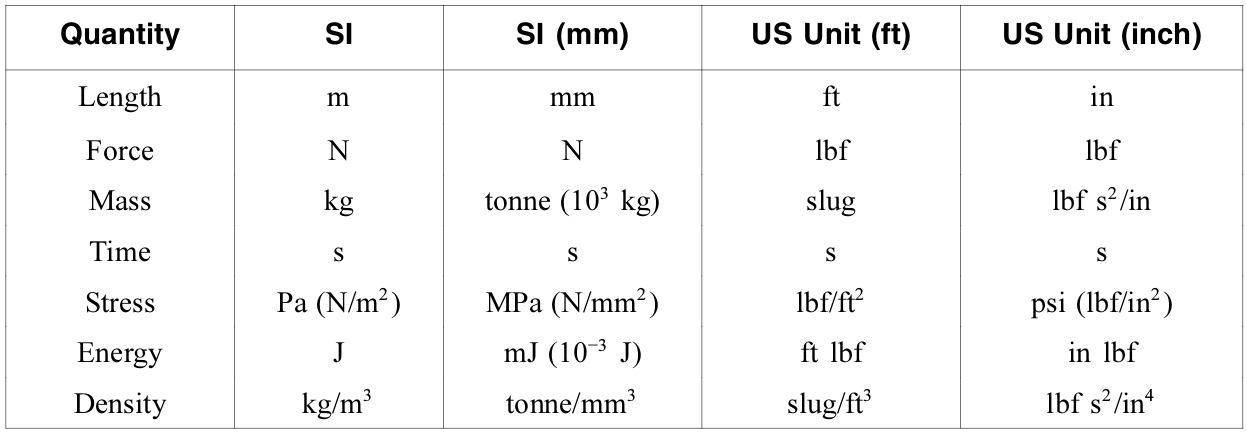
\includegraphics[width=0.9\textwidth]{./body/images/imagen01}
  \end{center}
  \caption{Unidades consistentes}
  \label{figu01}
\end{figure}

El problema que queremos resolver está resumido en la
Fig.~\ref{figu114}. Se trata de una ménsula empotrada en su extremo
izquierdo que tiene aplicada un vector tensión
$\mathbf{t}^*=[0,-1000,0]^T$ Pa en la mitad derecha de su cara
superior. Las medidas de la ménsula son 5 metros de largo y una
sección cuadrada de 1 metro de lado. El material es hormigón con
constantes elásticas $E=27$ GPa y $\nu=0.3$. Como puedes comprobar,
nuestro problema puede ser reducido a un problema plano en tensión
plana.
\begin{figure}[H]
  \begin{center}
    \includegraphics[width=0.9\textwidth]{./body/images/imagen114}
  \end{center}
  \caption{Descripción del modelo}
  \label{figu114}
\end{figure}



\paragraph{Inicio del análisis con Abaqus.} Antes de empezar a
trabajar hagamos tres cosas:
\begin{enumerate}
\item Definir un directorio de trabajo en \textbf{File/Set Working
    Directory} donde se guardarán todos los archivos que generemos.
\item Ver la ayuda de Abaqus:
  \begin{itemize}
  \item Si vas a \textbf{Help/On Context} obtendremos ayuda sobre
    aquel icono que pulsemos después.
  \item Si vas a \textbf{Help/On Module} obtendremos ayuda sobre el
    módulo en el que estés en ese momento.
  \item Si vas a \textbf{Help/Search and Browse Guide} iremos a la
    página principal de la ayuda de Abaqus.
  \end{itemize}
\item Asignemos un nombre a nuestro modelo.  Situamos el cursor encima
  del modelo en la parte superior del \textit{Model Tree}, pulsamos el
  botón derecho del ratón, seleccionamos \textbf{Rename} y le
  asignamos el nombre \textit{Mensula}. Tiene que quedarte como indica
  la Fig.~\ref{figu12}.
  \begin{figure}[H]
    \begin{center}
      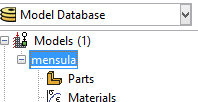
\includegraphics[width=0.3\textwidth]{./body/images/imagen12}
    \end{center}
    \caption{Cambio nombre del modelo}
    \label{figu12}
  \end{figure}
\end{enumerate}

A continuación vamos a describir todas las fases del análisis con la
ayuda del ejemplo descrito.
\clearpage

\subsection{Módulo Part. Crear la geometría de los elementos.}
En Abaqus debemos tener definida la geometría de los elementos que
forman nuestro modelo. Estos elementos se denominan \textit{parts} y
nos permitirán ensamblar luego un modelo creando una o varias copias
(instancias) de cada \textit{part}, en caso de que haya elementos
repetidos.

Para definir la geometría de los elementos de nuestro modelo:
\begin{enumerate}
\item Activamos primero el módulo \textbf{Part} y pulsamos el comando
  \textbf{Create Part} (Fig.~\ref{figu02}).

  En la esquina inferior izquierda Abaqus muestra un mensaje (Prompt)
  que nos indica qué tenemos que hacer. Pulsaremos el botón
  \textbf{Cancel} para cancelar la tarea que estamos haciendo, el
  botón \textbf{Previous} para cancelar el paso que estemos haciendo
  dentro de una tarea y volver al paso previo y el botón \textbf{Done}
  para acabar la tarea (ver Fig.~\ref{figu03}).

\begin{figure}[H]
  \centering
  \begin{subfigure}{0.25\textwidth}
    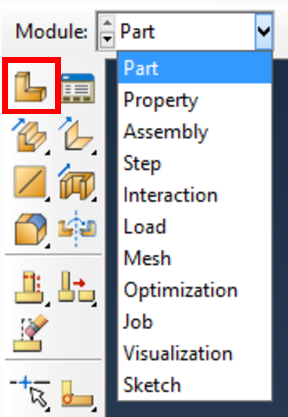
\includegraphics[width=\textwidth]{./body/images/imagen02.pdf}
    \caption{Comando \textbf{Create Part}}
    \label{figu02}
  \end{subfigure}%
  ~ %add desired spacing between images, e. g. ~, \quad, \qquad, \hfill etc.
  % (or a blank line to force the subfigure onto a new line)
  \begin{subfigure}{0.65\textwidth}
    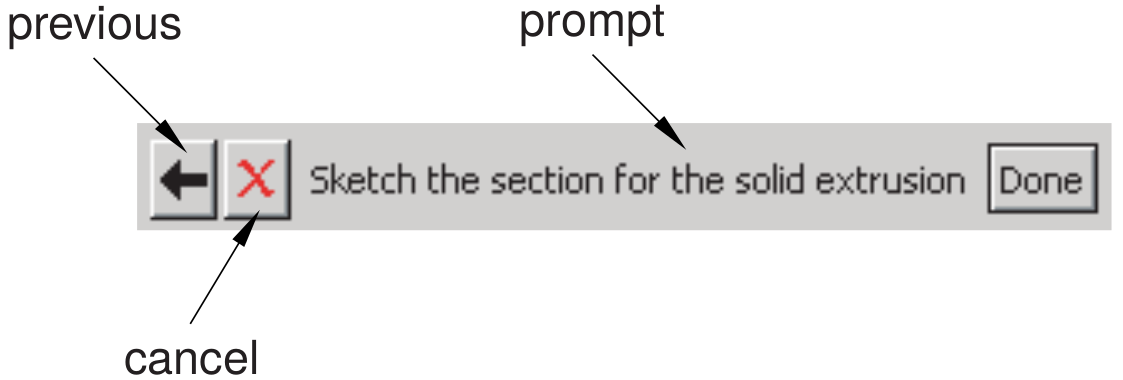
\includegraphics[width=\textwidth]{./body/images/imagen03}
    \caption{Mensaje que informa de la acción}
    \label{figu03}
  \end{subfigure}
  \caption{Inicio módulo part y mensaje \textit{Prompt} de
    información}
\end{figure}

Nos aparece el diálogo \textbf{Create Part} donde nos pregunta si va a
ser un dominio tridimensional, plano o axisimétrico (\textbf{Modeling
  Space}), si va a ser un objeto deformable o rígido (\textbf{type}) y
qué tipo de geometría es (\textbf{Base Feature}). Para nuestro
problema elegiremos las opciones que indica la Fig.~\ref{figu04}.
Para la variable \textbf{Approximante size} hemos puesto un valor de
10 (metros en nuestro sistema de unidades asumido), que es el doble de
la dimensión máxima de nuestro dominio y que Abaqus usará para
proporcionarnos un entorno de trabajo donde crear la geometría.
\begin{figure}[H]
  \begin{center}
    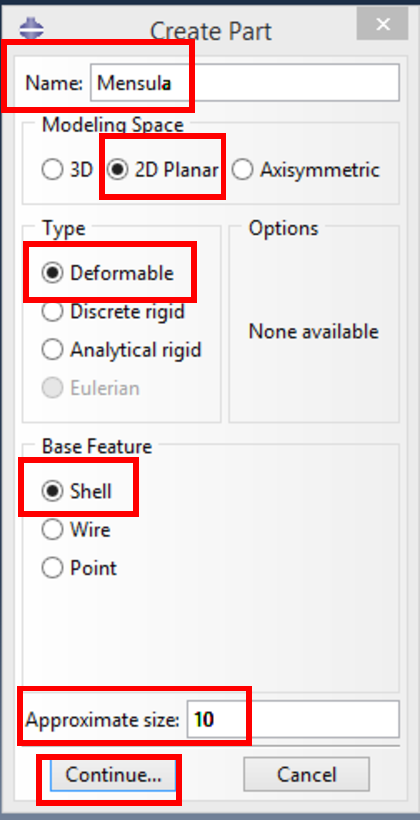
\includegraphics[width=0.35\textwidth]{./body/images/imagen04.pdf}
  \end{center}
  \caption{Diálogo \textbf{Create Part}}
  \label{figu04}
\end{figure}

\item A continuación nos aparece una pantalla de un entorno de trabajo
  (\textit{Sketcher}) con las herramientas CAD necesarias para crear
  la geometría de nuestra \textit{part}. Respecto al sketcher debemos
  saber:
  \begin{itemize}
  \item Puedes utilizar los puntos de la ventana de trabajo (pulsando
    con el ratón) para definir entidades geométricas.
  \item Las líneas punteadas son los ejes X e Y y se interseccionan en
    el origen.
  \item La orientación del plano de trabajo se define con los ejes de
    abajo a la izquierda.
  \item Cuando activas una herramienta de dibujo, las coordenadas se
    dibuja en la parte superior izquierda.
  \end{itemize}


  Hay dos caminos para definir dicha geometría: (a) definir de forma
  precisa las entidades geométricas y (b) definirlas rápidamente con el
  uso de la rejilla y luego aplicar restricciones para conseguir la
  geometría buscada. Vamos a trabajar de la segunda manera:
  \begin{enumerate}
  \item Pulsa el botón \textbf{Create lines: Rectangle} y dibuja un
    rectángulo sin preocuparte por las dimensiones (ver
    Fig.~\ref{figu05}).
    \begin{figure}[H]
      \begin{center}
        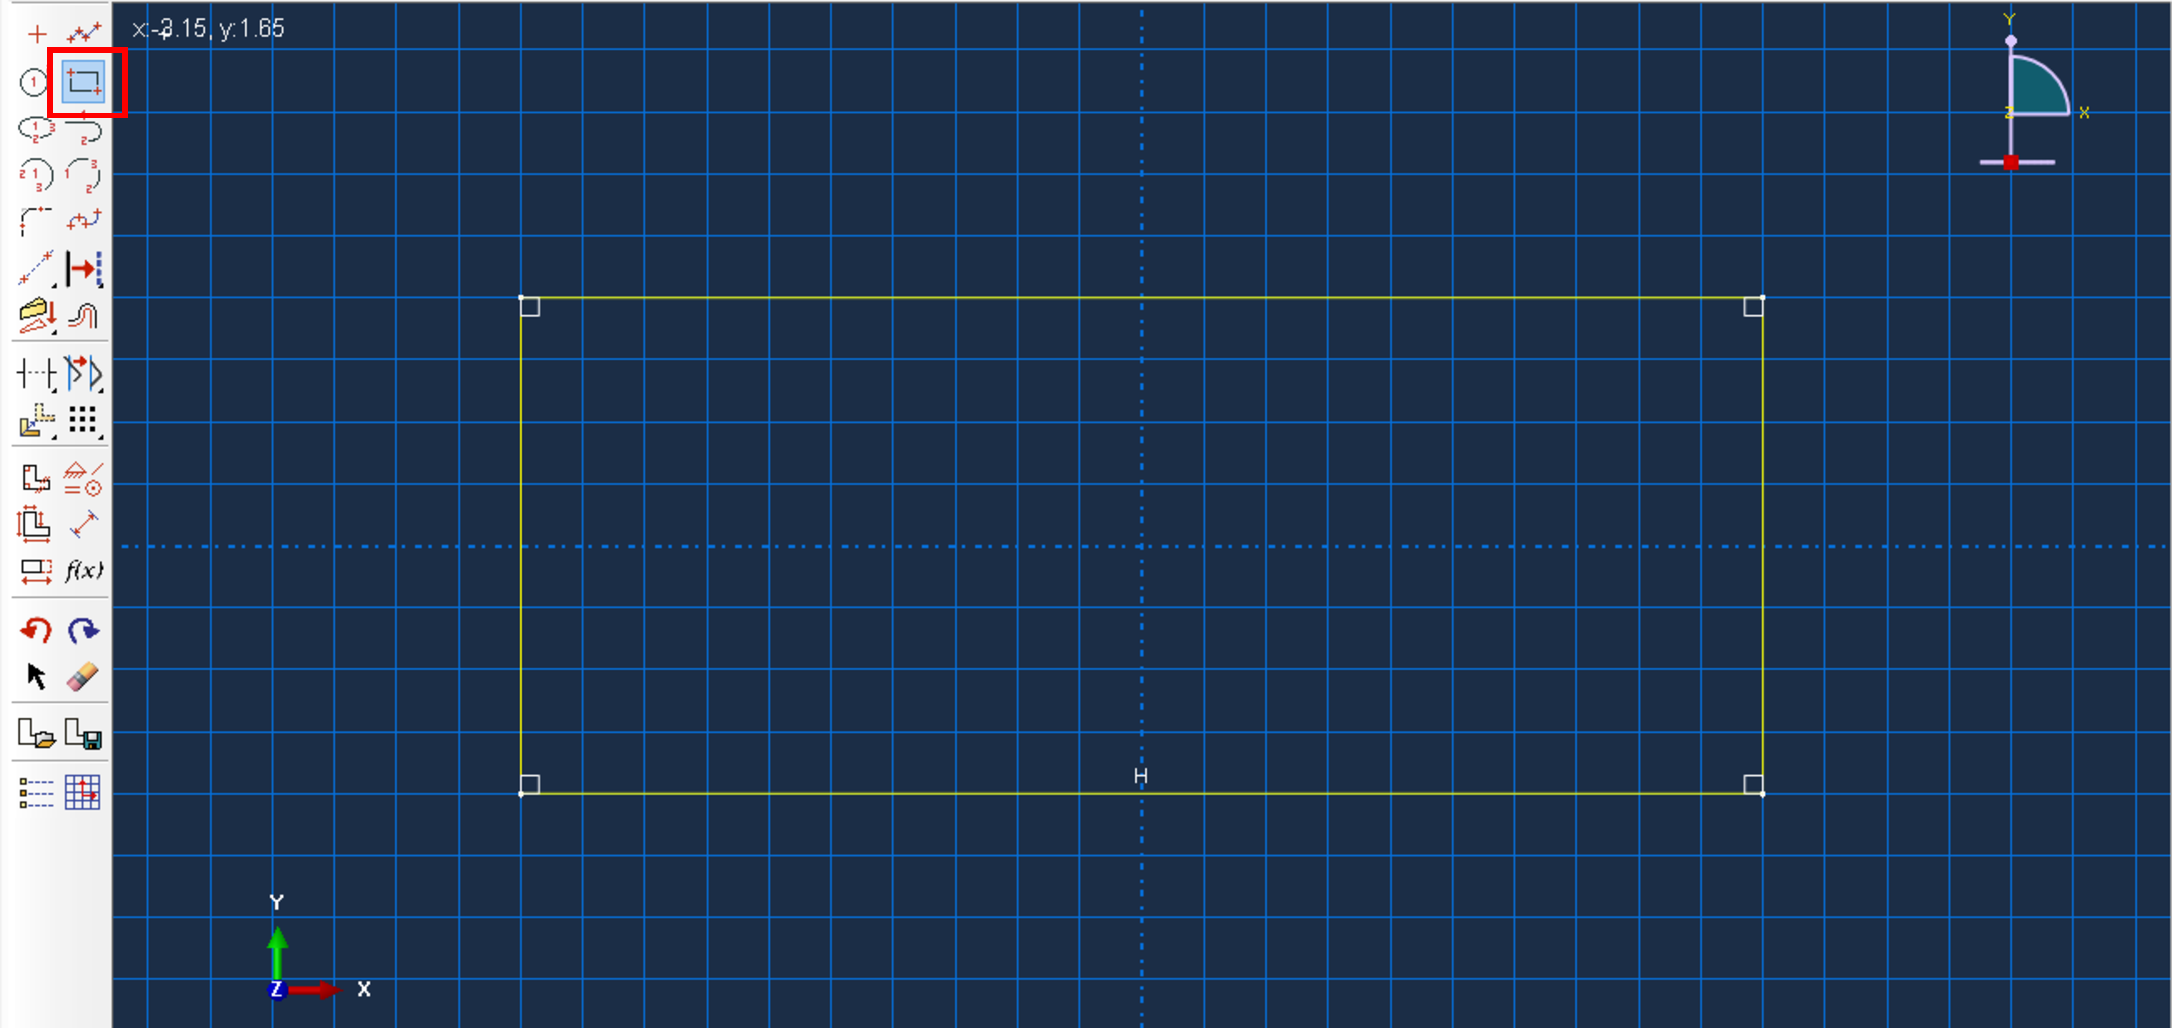
\includegraphics[width=0.875\textwidth]{./body/images/imagen05.pdf}
      \end{center}
      \caption{ Rectángulo inicial}
      \label{figu05}
    \end{figure}

  \item Pulsa el comando \textbf{Add dimension}, selecciona uno de los
    lados horizontales y modifica la dimensión a 5 metros (ver
    Fig.~\ref{figu06}).
    \begin{figure}[H]
      \begin{center}
        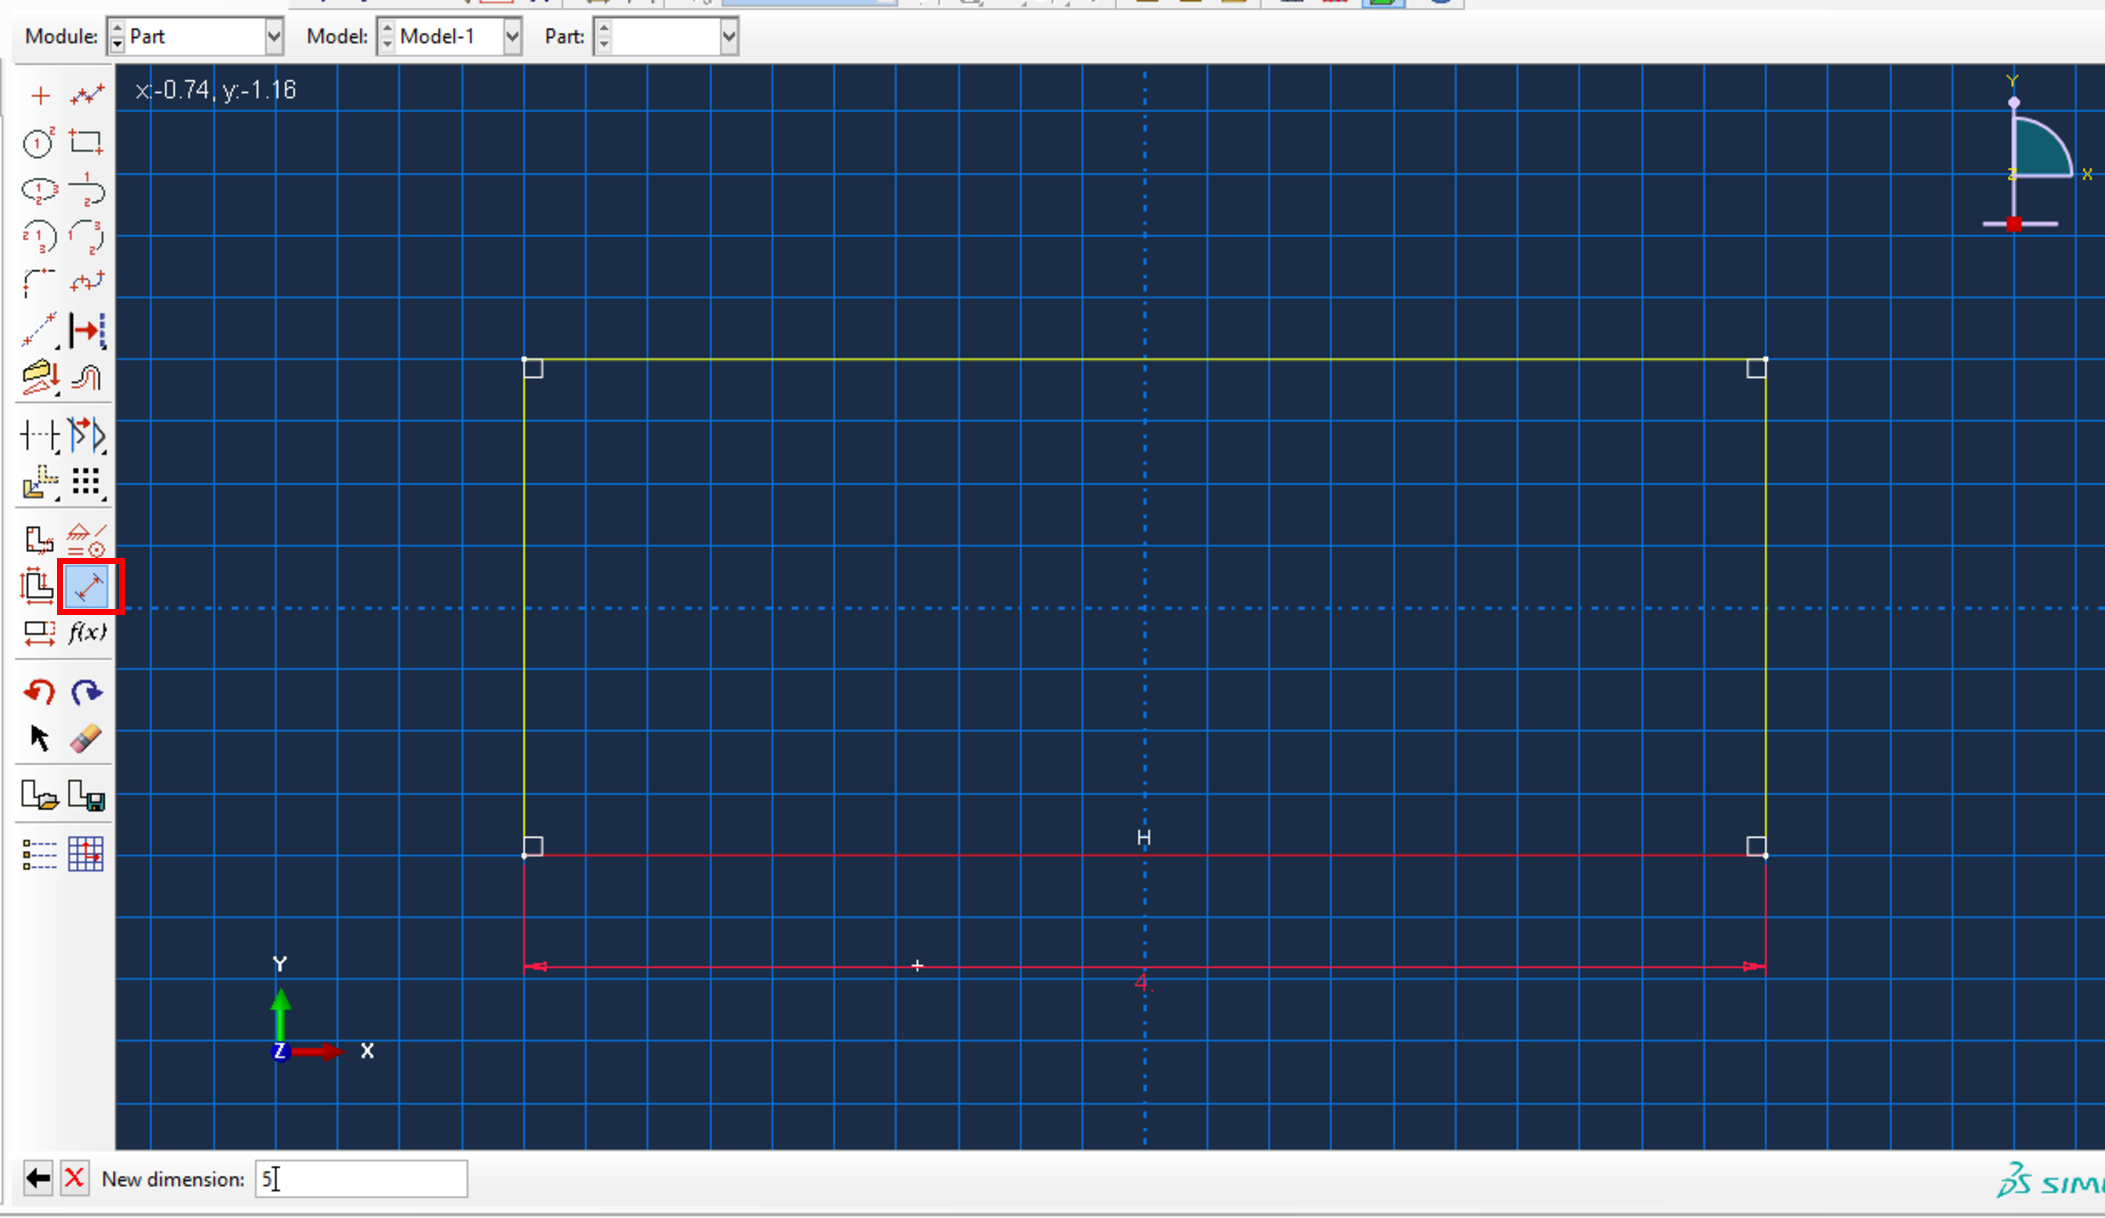
\includegraphics[width=0.875\textwidth]{./body/images/imagen06.pdf}
      \end{center}
      \caption{ Modificación de una dimensión}
      \label{figu06}
    \end{figure}

  \item Como en el apartado anterior modifica la dimensión vertical a
    1 metros. Una vez hecho, pulsa \textbf{Auto Fit view} para centrar
    la imagen (debe quedarte como la Fig.~\ref{figu07}).
    \begin{figure}[H]
      \begin{center}
        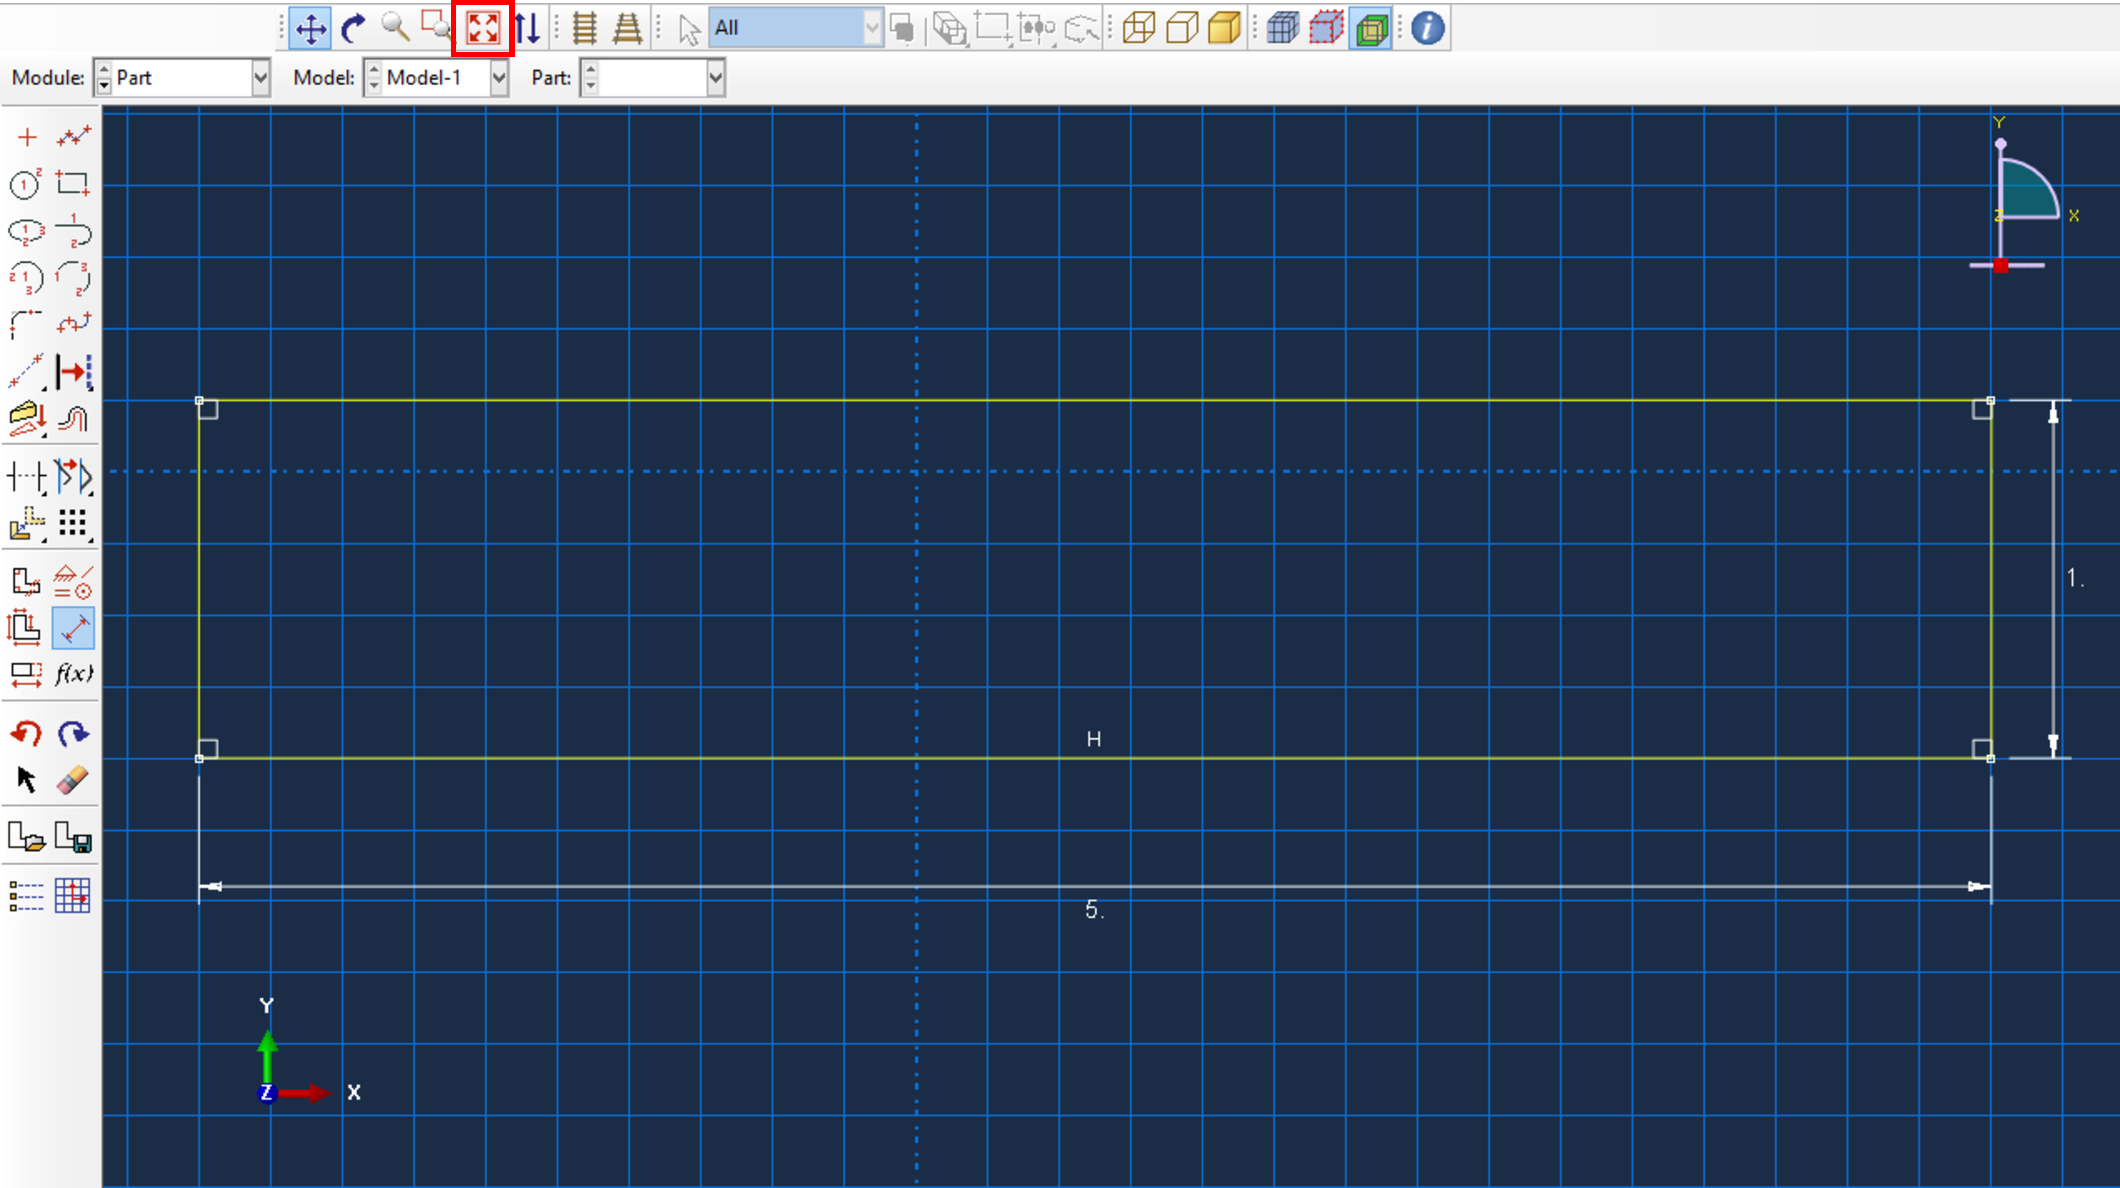
\includegraphics[width=0.875\textwidth]{./body/images/imagen07.pdf}
      \end{center}
      \caption{Rectángulo final}
      \label{figu07}
    \end{figure}

  \item Finalmente, pulsa cancel para abandonar la herramienta
    \textbf{Sketcher} y pulsa \textbf{Done} para generar la
    \textit{part} que buscábamos (ver Fig.~\ref{figu08}).
    \begin{figure}[H]
      \begin{center}
        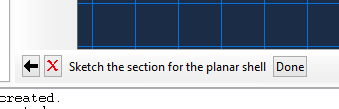
\includegraphics[width=0.55\textwidth]{./body/images/imagen08}
      \end{center}
      \caption{Orden final para crear el objeto \textit{Part}}
      \label{figu08}
    \end{figure}
  \end{enumerate}


\item Si nos fijamos en las cargas repartidas de nuestro modelo,
  debemos dividir el borde superior en dos mitades para poder asignar
  las cargas sólo en la mitad tal como indica la
  Fig.~\ref{figu114}. Para poder hacerlo sigue los siguientes pasos:
  \begin{enumerate}
  \item De los iconos asociados a la modificación de una
    \textit{part}, pulsa \textbf{Partition Edge: Enter Parameter} tal
    como indica la Fig.~\ref{figu34}. Posteriormente selecciona el
    borde superior de la ménsula (Fig.~\ref{figu35}).
    \begin{figure}[H]
      \centering
      \begin{subfigure}{0.29\textwidth}
        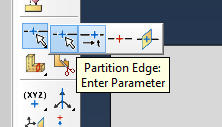
\includegraphics[width=\textwidth]{./body/images/imagen34}
        \caption{Activación \textbf{Partition Edge}}
        \label{figu34}
      \end{subfigure}%
      ~ %add desired spacing between images, e. g. ~, \quad, \qquad, \hfill etc.
      % (or a blank line to force the subfigure onto a new line)
      \begin{subfigure}{0.59\textwidth}
        
\includegraphics[width=\textwidth]{./body/images/imagen35}
        \caption{Selección borde superior}
        \label{figu35}
      \end{subfigure}%
      \caption{División de borde superior}
    \end{figure}
  \item A continuación nos pide un parámetro entre 0 y 1 para indicar
    el punto de corte según la dirección del vector que se ve en la
    pantalla. Como queremos dividir por la mitad, indica 0.5 tal como
    indica la Fig.~\ref{figu36}
    \begin{figure}[H]
      \begin{center}
        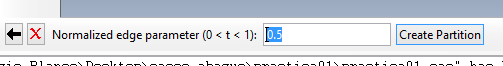
\includegraphics[width=0.75\textwidth]{./body/images/imagen36}
      \end{center}
      \caption{Introducción parámetro de división}
      \label{figu36}
    \end{figure}
  \end{enumerate}
\end{enumerate}
Una vez creada la \textit{Part}, guarda el modelo con la orden
\textbf{Save model database}.
\newpage

\subsection{Módulo Property. Definir materiales y secciones.}

En este módulo debemos definir los materiales, las secciones y asignar
esta información a la \textit{part} que hemos creado en el apartado
anterior.
\begin{enumerate}
\item \textbf{Definir el material.} Seleccionamos el módulo
  \textbf{Property} y pulsamos el icono \textbf{Create Material} (ver
  Fig.~\ref{figu13}). En la ventana que nos aparece para definir el
  material le damos un nombre, incluimos una breve descripción y le
  asignamos el comportamiento constitutivo mecánico \textbf{Elástico}
  tal como resume la Fig.~\ref{figu14}. Finalmente asigna las
  propiedades mecánicas de un hormigón estándar ($E=27$ GPa,
  $\nu=0.3$) como indica la Fig.~\ref{figu15}.

\begin{figure}[H]
  \centering
  \begin{subfigure}{0.19\textwidth}
    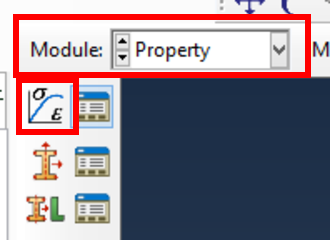
\includegraphics[width=\textwidth]{./body/images/imagen13.pdf}
    \caption{Comando \textbf{Create Material}}
    \label{figu13}
  \end{subfigure}%
  ~ %add desired spacing between images, e. g. ~, \quad, \qquad, \hfill etc.
  % (or a blank line to force the subfigure onto a new line)
  \begin{subfigure}{0.39\textwidth}
    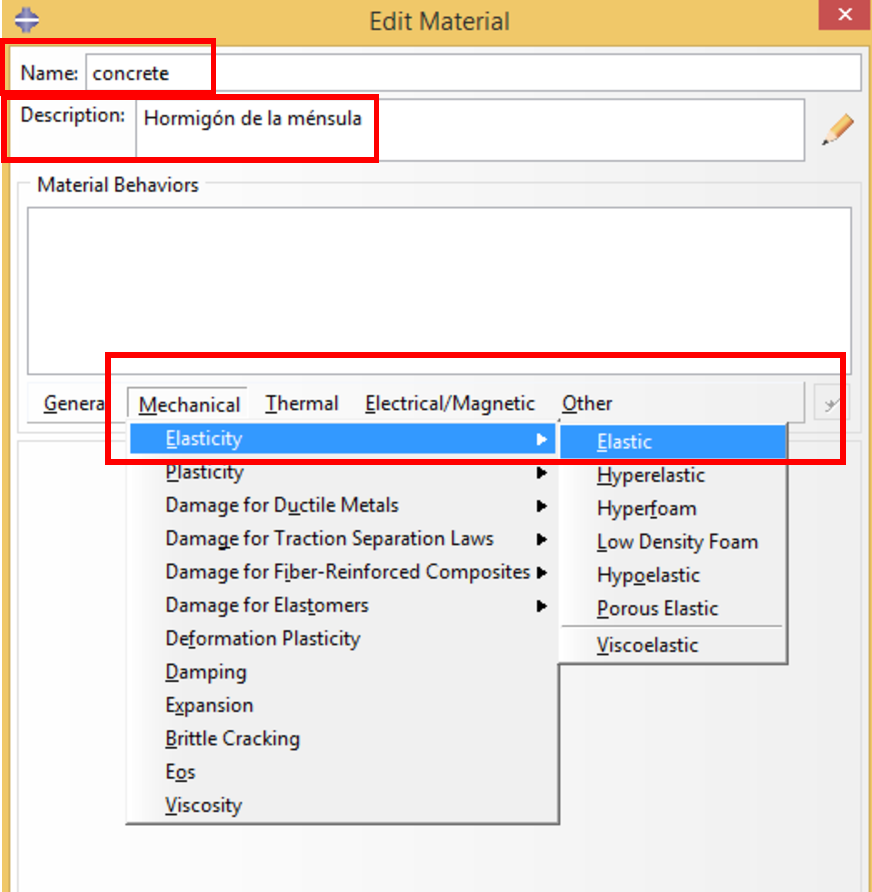
\includegraphics[width=\textwidth]{./body/images/imagen14.pdf}
    \caption{Selección tipo de comportamiento}
    \label{figu14}
  \end{subfigure}
  ~ %add desired spacing between images, e. g. ~, \quad, \qquad, \hfill etc.
  % (or a blank line to force the subfigure onto a new line)
  \begin{subfigure}{0.39\textwidth}
    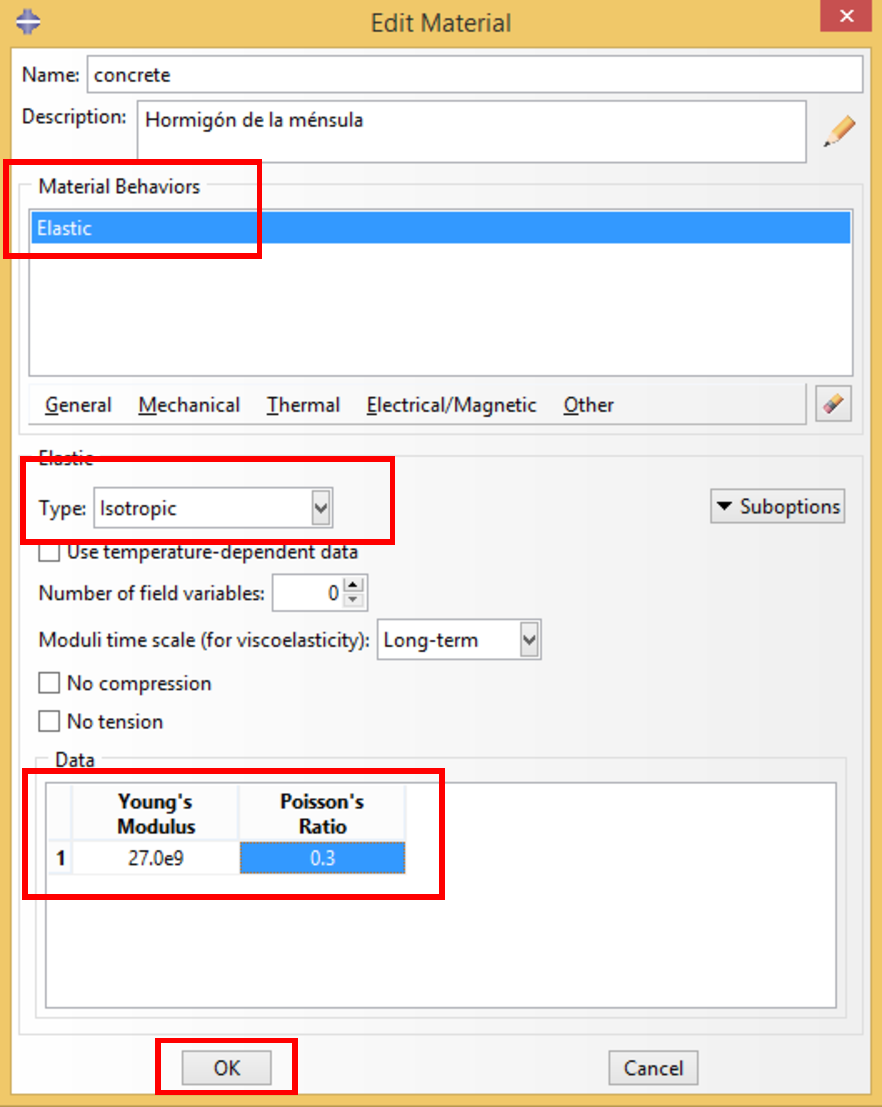
\includegraphics[width=\textwidth]{./body/images/imagen15.pdf}
    \caption{Definición parámetros del material}
    \label{figu15}
  \end{subfigure}
  ~ %add desired spacing between images, e. g. ~, \quad, \qquad, \hfill etc.
  % (or a blank line to force the subfigure onto a new line)
  \caption{Definición del material \textit{concrete}}
\end{figure}

\item \textbf{Definir la sección.} Aún dentro del módulo
  \textbf{Property} pulsamos el icono \textbf{Create Section} (ver
  Fig.~\ref{figu16}). En la siguiente ventana (Fig.~\ref{figu17})
  asignémosle el nombre \textit{SeccionMensula}, la categoría de
  elemento finito \textbf{Solid} y el tipo \textbf{Homogeneous}.
  Finalmente asociemos esta sección con el material concrete tal como
  indica la Fig.~\ref{figu18} (observa que el espesor por defecto de
  la pieza es 1 metro, que coincide con nuestra dimensión).
  \begin{figure}[H]
    \centering
    \begin{subfigure}{0.19\textwidth}
      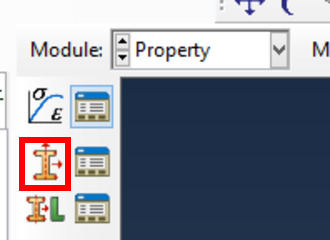
\includegraphics[width=\textwidth]{./body/images/imagen16.pdf}
      \caption{Comando \textbf{Create Section}}
      \label{figu16}
    \end{subfigure}%
    ~ %add desired spacing between images, e. g. ~, \quad, \qquad, \hfill etc.
    % (or a blank line to force the subfigure onto a new line)
    \begin{subfigure}{0.39\textwidth}
      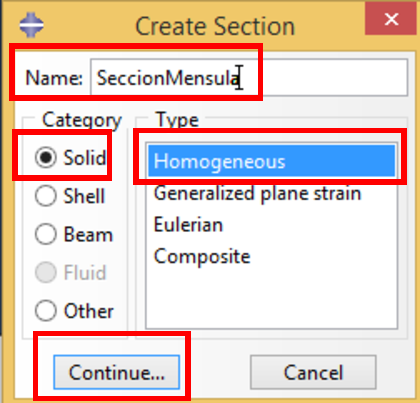
\includegraphics[width=\textwidth]{./body/images/imagen17.pdf}
      \caption{Definición propiedades de la sección}
      \label{figu17}
    \end{subfigure}
    ~ %add desired spacing between images, e. g. ~, \quad, \qquad, \hfill etc.
    % (or a blank line to force the subfigure onto a new line)
    \begin{subfigure}{0.39\textwidth}
      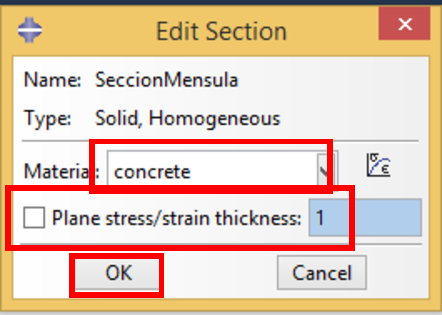
\includegraphics[width=\textwidth]{./body/images/imagen18.pdf}
      \caption{Asignación del material a la sección}
      \label{figu18}
    \end{subfigure}
    ~ %add desired spacing between images, e. g. ~, \quad, \qquad, \hfill etc.
    % (or a blank line to force the subfigure onto a new line)
    \caption{Definición de la sección \textit{SeccionMensula}}
  \end{figure}


\item \textbf{Asignar la sección a una part.}  Finalmente, en este
  módulo debemos asignar la anterior sección a la \textit{part}
  creada. Para ello pulsamos el icono \textbf{Assign Section} (ver
  Fig.~\ref{figu21} y seleccionamos la región a la que queremos
  asignar la sección (la ménsula). Le decimos que le queremos asignar
  la sección \textit{SeccionMénsula} (ver Fig.~\ref{figu19}) y nuestra
  \textit{part} deberá haber cambiado de color tal como indica la
  Fig.~\ref{figu20}
  \begin{figure}[H]
    \centering
    \begin{subfigure}{0.19\textwidth}
      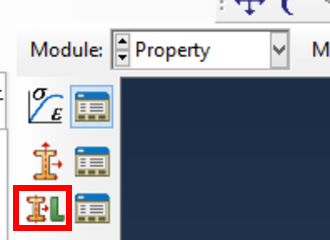
\includegraphics[width=\textwidth]{./body/images/imagen21.pdf}
      \caption{Comando \textbf{Assign Section}}
      \label{figu21}
    \end{subfigure}%
    ~ %add desired spacing between images, e. g. ~, \quad, \qquad, \hfill etc.
    % (or a blank line to force the subfigure onto a new line)
    \begin{subfigure}{0.29\textwidth}
      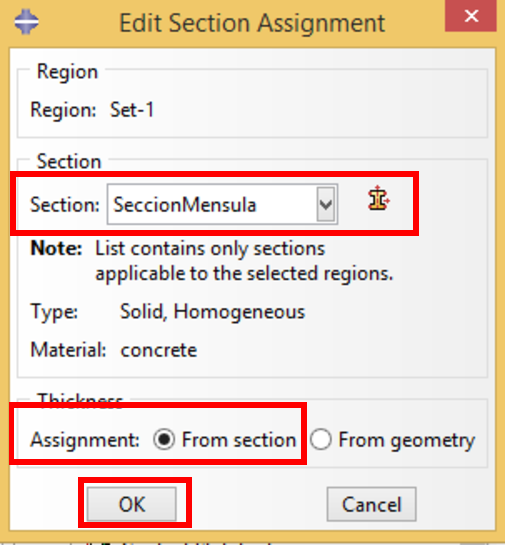
\includegraphics[width=\textwidth]{./body/images/imagen19.pdf}
      \caption{Vinculación sección a Part}
      \label{figu19}
    \end{subfigure}%
    ~ %add desired spacing between images, e. g. ~, \quad, \qquad, \hfill etc.
    % (or a blank line to force the subfigure onto a new line)
    \begin{subfigure}{0.49\textwidth}
      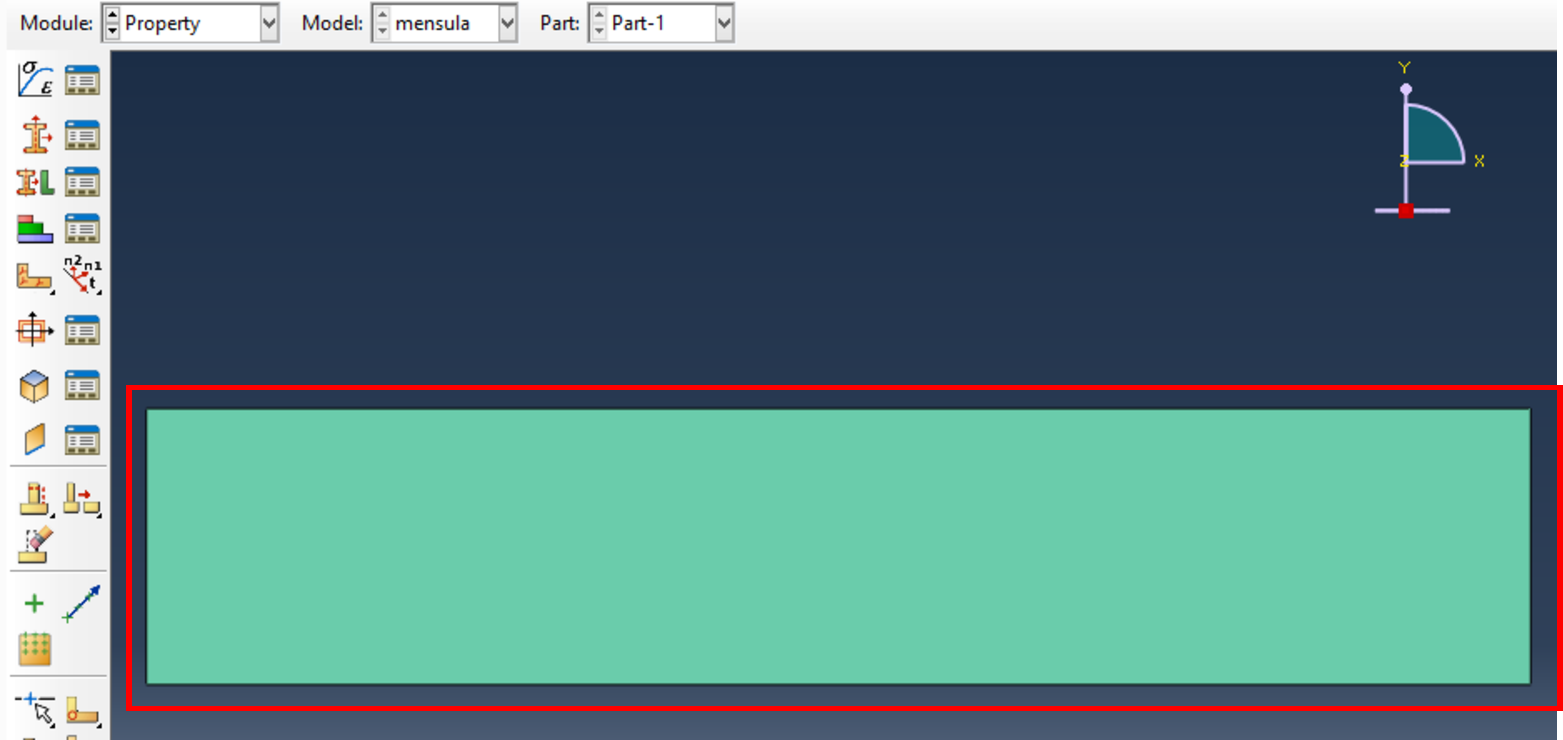
\includegraphics[width=\textwidth]{./body/images/imagen20.pdf}
      \caption{Part con sección asignada}
      \label{figu20}
    \end{subfigure}
    \caption{Asignación de la sección a una \textit{Part}}
  \end{figure}
\end{enumerate}
\newpage
\subsection{Módulo Assembly. Ensamblar el modelo}

Todo modelo de Abaqus se construye como un conjunto de copias
(\textit{instances}) de las \textit{parts} creadas. Nuestro problema
es muy sencillo y simplemente debemos crear un conjunto
(\textit{Assembly}) con una única copia de nuestra \textit{part}.  Sin
embargo imagina que quisiéramos modelar un coche, y que hemos ido
creando \textit{parts} de sus distintas componentes. Con la lógica de
Abaqus habríamos creado una \textit{part} definiendo una rueda, y en el
momento de crear el modelo final, haríamos cuatro copias de esa
\textit{part} para cada una de las ruedas del coche.

Para montar el modelo sigue los pasos que se indican a continuación:
\begin{enumerate}
\item Activa el módulo \textbf{Assembly} y pulsa el icono
  \textbf{Create instance} tal como indica la Fig.~\ref{figu22}
\item En la caja de diálogo que aparece (ver Fig.~\ref{figu23}),
  selecciona la \textit{part} de la que vamos a hacer copia (sólo hay
  una) e indica que la copia será de tipo \textbf{Dependent}
  (definiremos la malla en la \textit{part} y ésta se replicará en la
  copia que estamos creando)
\end{enumerate}

\begin{figure}[H]
  \centering
  \begin{subfigure}[H]{0.25\textwidth}
    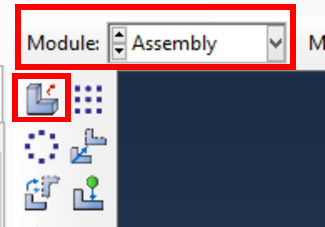
\includegraphics[width=\textwidth]{./body/images/imagen22.pdf}
    \caption{Comando \textbf{Create instance}}
    \label{figu22}
  \end{subfigure}%
  ~ %add desired spacing between images, e. g. ~, \quad, \qquad, \hfill etc.
  % (or a blank line to force the subfigure onto a new line)
  \begin{subfigure}{0.42\textwidth}
    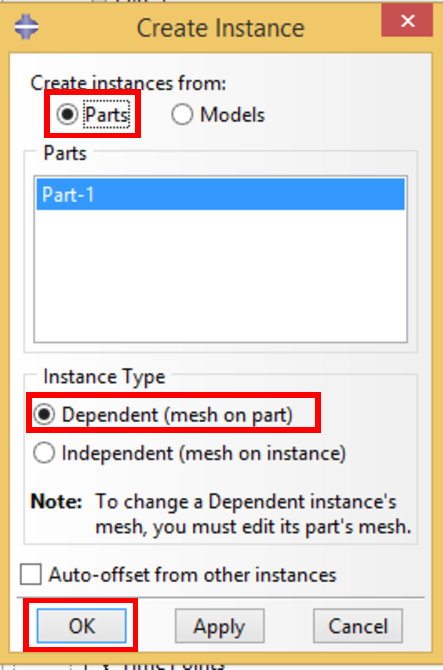
\includegraphics[width=\textwidth]{./body/images/imagen23.pdf}
    \caption{Creación de una copia \textit{Dependiente}}
    \label{figu23}
  \end{subfigure}%
  \caption{Acción \textbf{Create Instance}}
\end{figure}

Para facilitarnos operaciones posteriores, Abaqus nos permite agrupar
puntos nodales de entidades geométricas en elementos llamados
\textbf{sets}. De esta forma cuando queramos obtener los resultados en
esa entidad geométrica se lo podremos solicitar a Abaqus sin necesidad
de conocer los nodos de la malla que la forman. En nuestro caso vamos
a querer conocer la distribución de las fuerzas nodales en el extremo
empotrado de la viga. Por ello vamos a crear un set de los futuros
nodos de la malla en esta geometría:
\begin{enumerate}
\item Para crear un set haz doble click con el ratón sobre el elemento
  \textbf{Sets} en el \textbf{Model Tree} (ver Fig.~\ref{figu24}) o
  bien pulsa \textbf{Tools/Set/Create} (ver Fig.~\ref{figu25}).
  \begin{figure}[H]
    \centering
    \begin{subfigure}{0.35\textwidth}
      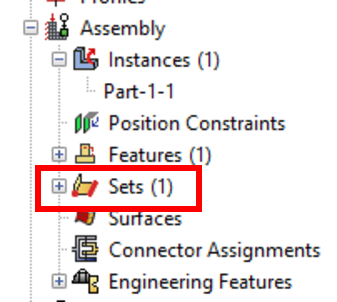
\includegraphics[width=\textwidth]{./body/images/imagen24.pdf}
      \caption{\textbf{Model Tree}}
      \label{figu24}
    \end{subfigure}%
    ~ %add desired spacing between images, e. g. ~, \quad, \qquad, \hfill etc.
    % (or a blank line to force the subfigure onto a new line)
    \begin{subfigure}{0.40\textwidth}
      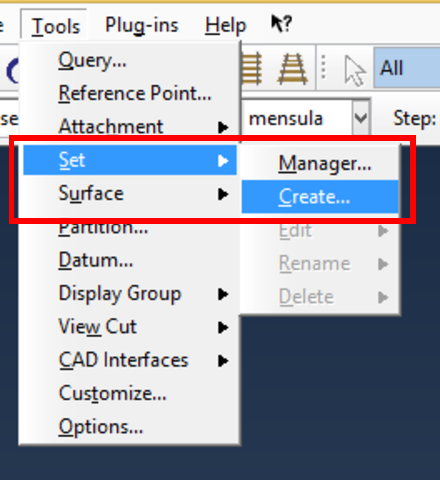
\includegraphics[width=\textwidth]{./body/images/imagen25.pdf}
      \caption{Inicio creación \textbf{set}}
      \label{figu25}
    \end{subfigure}%
    \caption{Creación de un \textbf{set}}
  \end{figure}
\item Asígnale el nombre \textit{LadoIzquierdo} en la siguiente
  ventana (ver Fig.~\ref{figu26}) y selecciona el lado izquierdo de la
  ménsula (ver Fig.~\ref{figu27}).
  \begin{figure}[H]
    \centering
    \begin{subfigure}{0.25\textwidth}
      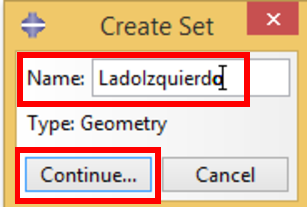
\includegraphics[width=\textwidth]{./body/images/imagen26.pdf}
      \caption{Asignación nombre al set}
      \label{figu26}
    \end{subfigure}%
    ~ %add desired spacing between images, e. g. ~, \quad, \qquad, \hfill etc.
    % (or a blank line to force the subfigure onto a new line)
    \begin{subfigure}{0.28\textwidth}
      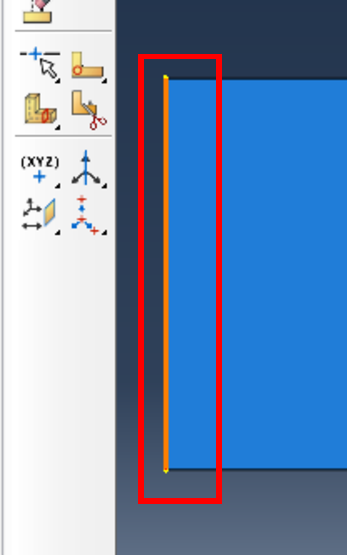
\includegraphics[width=\textwidth]{./body/images/imagen27.pdf}
      \caption{Selección del borde izquierdo}
      \label{figu27}
    \end{subfigure}%
    \caption{Creación de un \textbf{set}}
  \end{figure}
\item Asegúrate que en el \textbf{Model Tree} se ha creado un nuevo
  set tal como indica la Fig.~\ref{figu28})
  \begin{figure}[H]
    \centering
    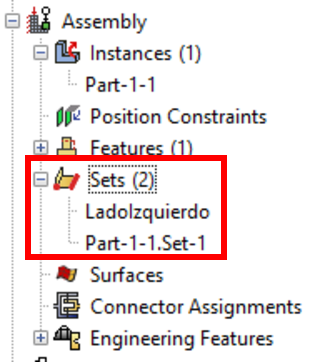
\includegraphics[width=0.39\textwidth]{./body/images/imagen28.pdf}
    \caption{\textbf{Model Tree} con dos sets}
    \label{figu28}
  \end{figure}
\end{enumerate}
\newpage
\subsection{Módulo Step. Configurar el procedimiento de análisis.}
Una vez construido el modelo, debemos definir en Abaqus los pasos de
cálculo (\textbf{steps}) que vamos a utilizar en nuestro análisis y
qué información queremos guardar de cada uno. Abaqus define un paso de
cálculo \textit{Initial} que asumiremos es el inicio de nuestro
análisis y donde aplicaremos la condición de contorno en
desplazamientos (el empotramiento).  Para aplicar el vector tensión
impuesto definiremos un único paso de cálculo y haremos un análisis
estático. Para definir el paso de cálculo (\textbf{Step}) sigue
los siguientes pasos.
\begin{enumerate}
\item Activa el módulo \textbf{Step} y pulsa el icono \textbf{Create
    Steps} tal como indica la Fig.~\ref{figu29}. En el cuadro de
  diálogo que te aparece (ver Fig.~\ref{figu30} ) nombra el caso como
  \textit{CasoEstatico} e indica que el análisis es de tipo
  \textbf{Static, General}.
  \begin{figure}[H]
    \centering
    \begin{subfigure}{0.29\textwidth}
      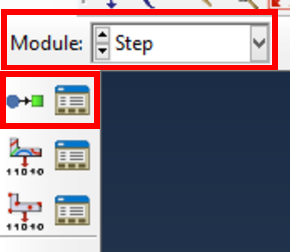
\includegraphics[width=\textwidth]{./body/images/imagen29.pdf}
      \caption{Comando \textbf{Create Steps}}
      \label{figu29}
    \end{subfigure}%
    ~ %add desired spacing between images, e. g. ~, \quad, \qquad, \hfill etc.
    % (or a blank line to force the subfigure onto a new line)
    \begin{subfigure}{0.40\textwidth}
      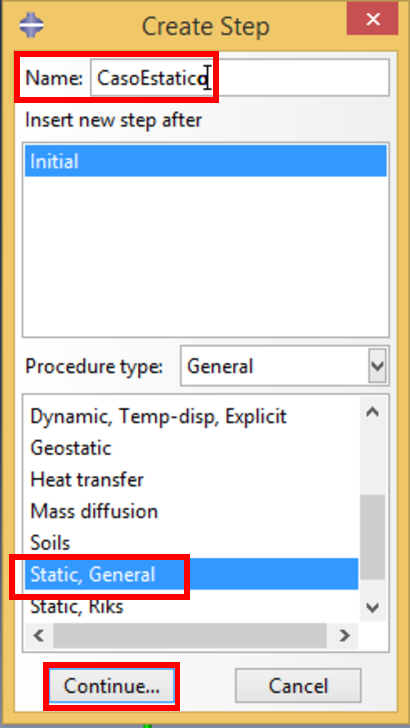
\includegraphics[width=\textwidth]{./body/images/imagen30.pdf}
      \caption{Propiedades nuevo paso de cálculo}
      \label{figu30}
    \end{subfigure}%
    \caption{Creación de nuevo paso de cálculo}
  \end{figure}
\item Ahora vamos a definir qué información queremos que nos guarde en
  el paso de cálculo creado para poder analizarla en el
  postproceso. Bajo el nombre \textbf{Field Output} Abaqus guarda la
  información de la solución en el dominio en un instante
  dado. Selecciona el icono \textbf{Create Field Output} (ver
  Fig.~\ref{figu31}) para crear un nuevo campo de resultados. En el
  siguiente diálogo nómbralo \textit{F-Output-Nuevo} y asígnalo al
  intervalo que acabamos de crear \textit{CasoEstatico} (ver
  Fig.~\ref{figu32}). De los campos disponibles para el postproceso
  elegiremos el tensor de tensiones (S), la tensión equivalente de von
  Mises (MISES), los desplazamientos (U), las fuerzas de reacción y
  momentos (RF) y las fuerzas y momentos concentrados (CF) tal como
  indica la Fig.~\ref{figu33}.
  \begin{figure}[H]
    \centering
    \begin{subfigure}{0.25\textwidth}
      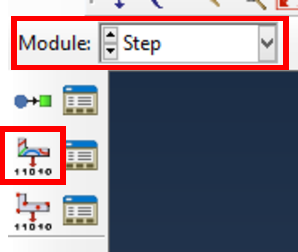
\includegraphics[width=\textwidth]{./body/images/imagen31.pdf}
      \caption{Crear nuevo \textbf{Field Output}}
      \label{figu31}
    \end{subfigure}%
    ~ %add desired spacing between images, e. g. ~, \quad, \qquad, \hfill etc.
    % (or a blank line to force the subfigure onto a new line)
    \begin{subfigure}{0.33\textwidth}
      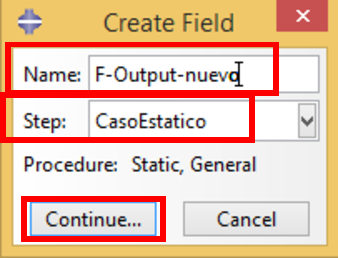
\includegraphics[width=\textwidth]{./body/images/imagen32.pdf}
      \caption{Asignación del \textbf{Field Output} al \textbf{Step}}
      \label{figu32}
    \end{subfigure}%
    ~ %add desired spacing between images, e. g. ~, \quad, \qquad, \hfill etc.
    % (or a blank line to force the subfigure onto a new line)
    \begin{subfigure}{0.40\textwidth}
      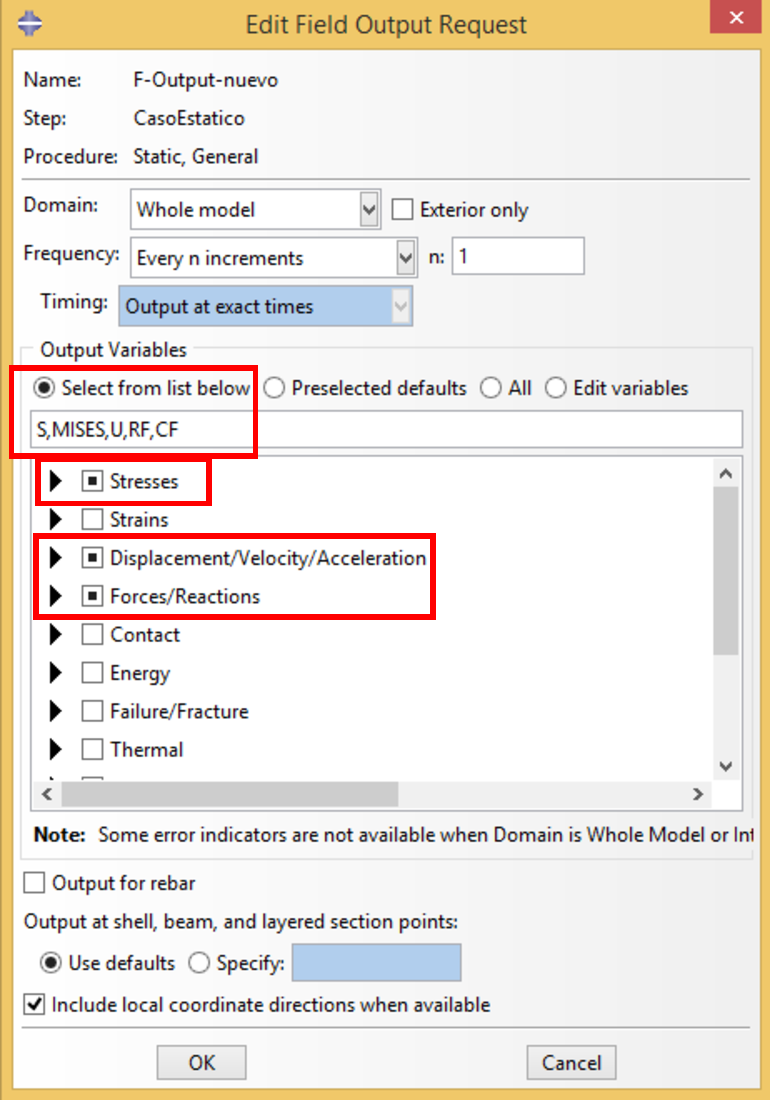
\includegraphics[width=\textwidth]{./body/images/imagen33.pdf}
      \caption{Definición componentes del \textbf{Field Output}}
      \label{figu33}
    \end{subfigure}%
    \caption{Definición de \textbf{Field Output}}
  \end{figure}
\item Bajo el nombre \textbf{History Output} Abaqus guarda la
  información de la solución en un punto durante un intervalo de
  tiempo. Como estamos en un problema cuasi-estático no nos interesa
  la evolución temporal de una variable y vamos a eliminar la que
  Abaqus crea por defecto. Para hacerlo pulsa el botón derecho del
  ratón sobre el nodo \textbf{History Output Request} del
  \textbf{Model Tree} y selecciona \textbf{Manager} tal como indica la
  Fig.~\ref{figu41}. Nos aparecerá una ventana con el gestor de
  variables históricas (ver Fig.~\ref{figu42}), selecciona la variable
  \textbf{H-Output-1} y pulsa \textbf{Delete}.
  \begin{figure}[H]
    \centering
    \begin{subfigure}{0.45\textwidth}
      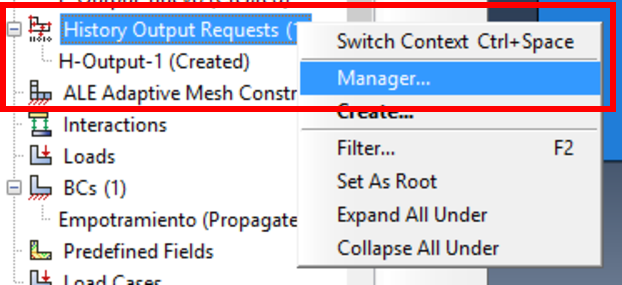
\includegraphics[width=\textwidth]{./body/images/imagen41.pdf}
      \caption{Apertura Gestor de \textbf{History Outputs}}
      \label{figu41}
    \end{subfigure}%
    ~ %add desired spacing between images, e. g. ~, \quad, \qquad, \hfill etc.
    % (or a blank line to force the subfigure onto a new line)
    \begin{subfigure}{0.45\textwidth}
      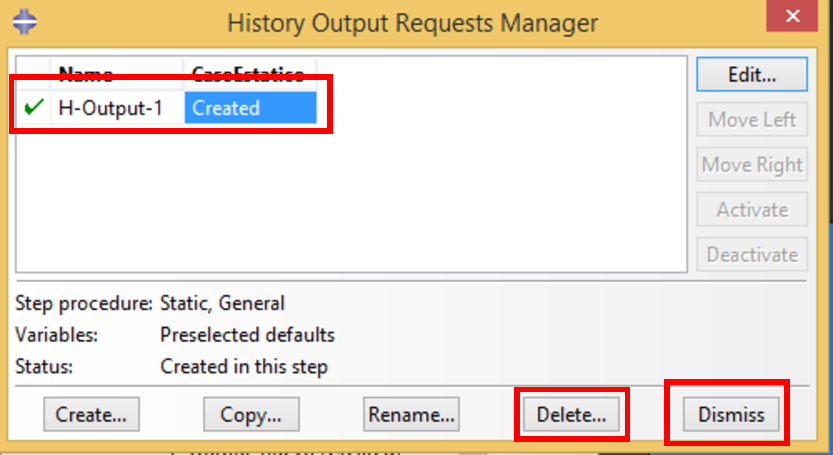
\includegraphics[width=\textwidth]{./body/images/imagen42.pdf}
      \caption{Gestor de \textbf{History Outputs}}
      \label{figu42}
    \end{subfigure}%
    \caption{Eliminación de las \textbf{History Outputs}}
  \end{figure}
\end{enumerate}
\newpage
\subsection{Módulo Load. Aplicar las condiciones de contorno}

Las condiciones de contorno que queremos aplicar son esenciales
(imponemos que el desplazamiento es nulo en el empotramiento) y naturales
(imponemos un vector tensión $\textbf{t}^*$ en el la
mitad derecha de parte superior de la ménsula). El empotramiento lo
aplicaremos en el paso de cálculo \textit{Initial} y el vector
tensión en el paso de cálculo creado \textit{CasoEstatico}.


Para imponer la condición de contorno esencial haz como sigue:
\begin{enumerate}
\item Activa el módulo load y pulsa \textbf{Create Boundary Condition}
  (ver Fig.\ref{figu37}).
  \begin{figure}[H]
    \centering
    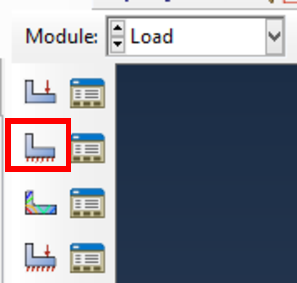
\includegraphics[width=0.33\textwidth]{./body/images/imagen37.pdf}
    \caption{Comando \textbf{Create Boundary Condition}}
    \label{figu37}
  \end{figure}
\item En el cuadro de diálogo que aparece (ver Fig.\ref{figu38}), pon
  el nombre \textit{Empotramiento} a la condición de contorno,
  asígnalo al paso de cálculo \textbf{Initial}, indica que es de la
  categoría \textbf{Mechanical} y que va a ser de tipo
  \textbf{Symmetry/Antisymmetry/Encastre}. Selecciona el lado izquierdo donde impondremos la condición de contorno. En el siguiente cuadro
  indica que la condición de contorno es de tipo \textbf{Encastre}
  (empotramiento) tal como indica la Fig.~\ref{figu39}.
  \begin{figure}[H]
    \centering
    \begin{subfigure}{0.45\textwidth}
      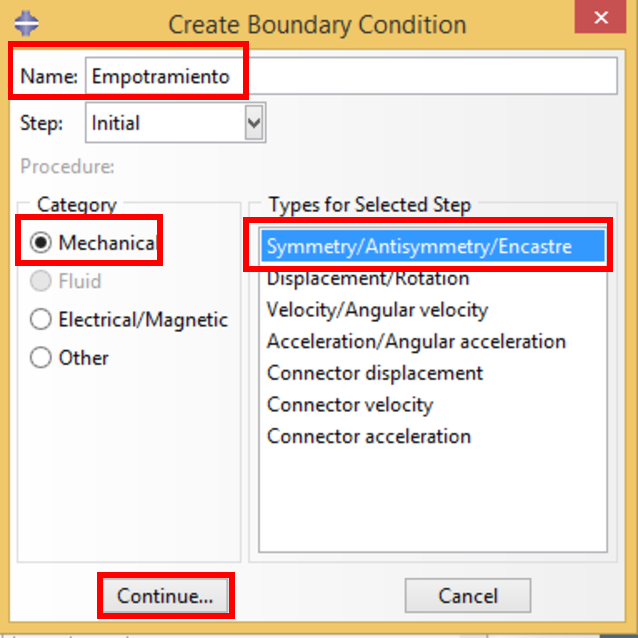
\includegraphics[width=\textwidth]{./body/images/imagen38.pdf}
      \caption{Creación de la condición de contorno}
      \label{figu38}
    \end{subfigure}%
    ~ %add desired spacing between images, e. g. ~, \quad, \qquad, \hfill etc.
    % (or a blank line to force the subfigure onto a new line)
    \begin{subfigure}{0.45\textwidth}
      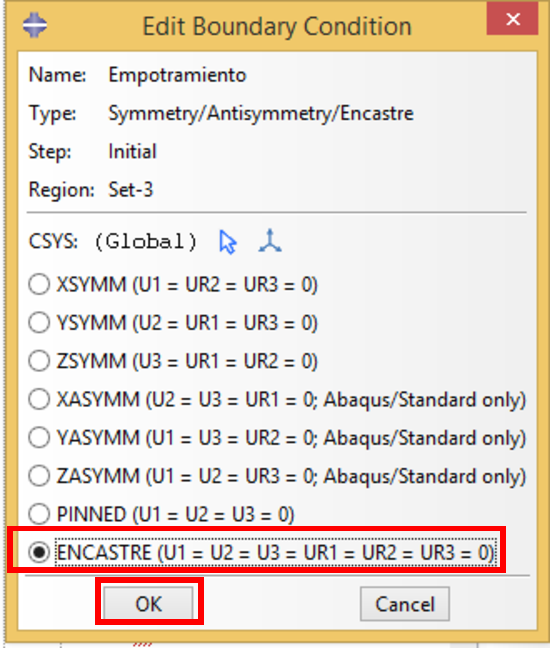
\includegraphics[width=\textwidth]{./body/images/imagen39.pdf}
      \caption{Edición de la condición de contorno}
      \label{figu39}
    \end{subfigure}%
    \caption{Definición de la condición de contorno de empotramiento}
  \end{figure}
\item Finalmente nos tiene que aparece en la pantalla de trabajo (ver
  Fig.\ref{figu40}) nuestro modelo con la representación de los grados
  de libertad impuestos a cero.
  \begin{figure}[H]
    \centering
    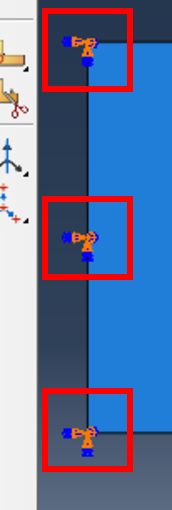
\includegraphics[width=0.19\textwidth]{./body/images/imagen40.pdf}
    \caption{Detalle condición de contorno de empotramiento}
    \label{figu40}
  \end{figure}
\end{enumerate}


Para imponer la condición de contorno natural haz como sigue:
\begin{enumerate}
\item Pulsa el icono \textbf{Create Load} tal como indica la
  Fig.~\ref{figu43}. En el cuadro de diálogo que aparece (ver
  Fig.~\ref{figu44}) nombra la condición de contorno como
  \textit{CargaRepartida}, aplícala en el paso de cálculo
  \textit{CasoEstatico}, indica que su categoría es
  \textbf{Mechanical} y el tipo \textbf{Surface traction}. Selecciona
  la mitad derecha del borde superior de la ménsula tal como
  describe la Fig.~\ref{figu45}.
  \begin{figure}[H]
    \centering
    \begin{subfigure}{0.23\textwidth}
      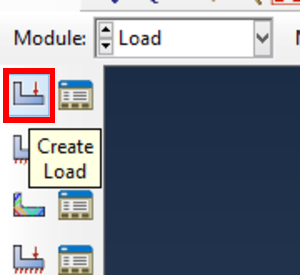
\includegraphics[width=\textwidth]{./body/images/imagen43.pdf}
      \caption{Comando \textbf{Create Load}}
      \label{figu43}
    \end{subfigure}%
    ~ %add desired spacing between images, e. g. ~, \quad, \qquad, \hfill etc.
    % (or a blank line to force the subfigure onto a new line)
    \begin{subfigure}{0.30\textwidth}
      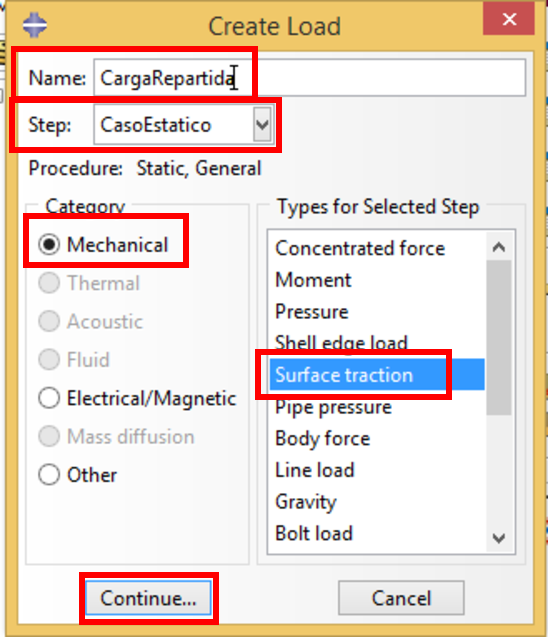
\includegraphics[width=\textwidth]{./body/images/imagen44.pdf}
      \caption{Tipo de carga aplicar}
      \label{figu44}
    \end{subfigure}%
    ~ %add desired spacing between images, e. g. ~, \quad, \qquad, \hfill etc.
    % (or a blank line to force the subfigure onto a new line)
    \begin{subfigure}{0.44\textwidth}
      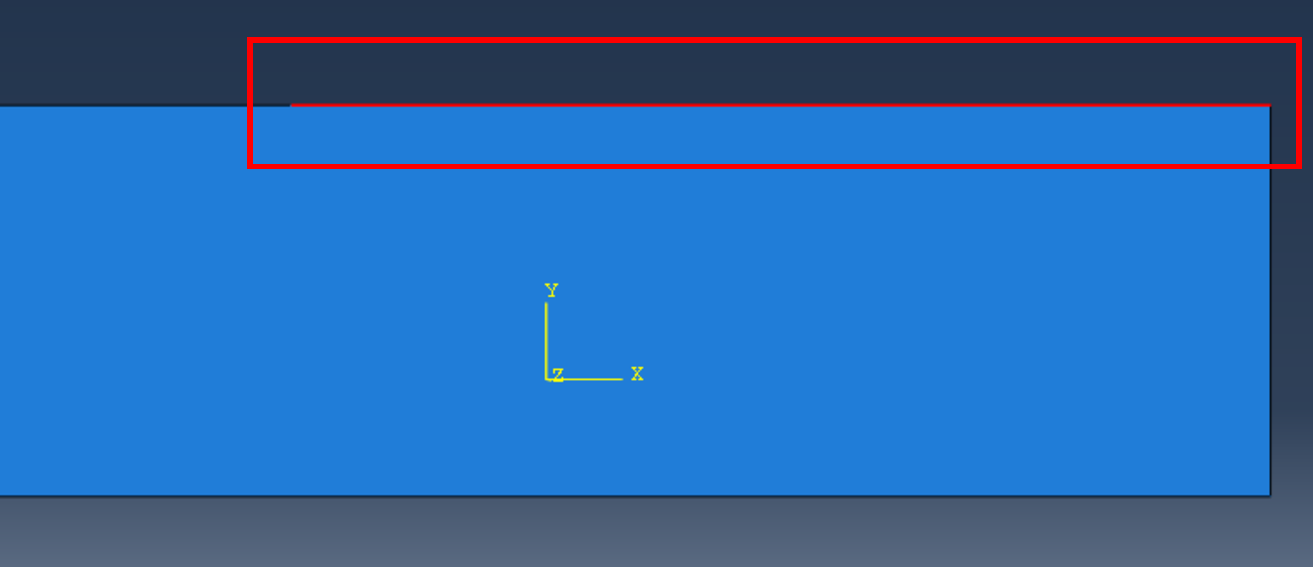
\includegraphics[width=\textwidth]{./body/images/imagen45.pdf}
      \caption{Selección borde superior derecho}
      \label{figu45}
    \end{subfigure}%
    \caption{Definición carga repartida (I)}
  \end{figure}
\item El siguiente cuadro de diálogo nos permite definir el vector
  tensión. Indica que es de tipo \textbf{General} y de módulo 1000 Pa
  (ver Fig.~\ref{figu46}). Es necesario definir la dirección y el
  sentido del vector tensión. Pulsa en la flecha azul junto a la
  palabra \textbf{Vector} para definir un vector que nos proporcione
  la dirección y el sentido del vector tensión (no tiene que ser
  unitario). Se puede hacer pulsando dos vértices de nuestra geometría
  o introduciendo dos pares de coordenadas. Vamos a hacerlo de la
  última forma. Introduce en la parte inferior izquierda las
  coordenadas del punto inicial (Fig.~\ref{figu47}, luego pulsa intro)
  y del punto final (Fig.~\ref{figu48}, luego pulsa intro).

\begin{figure}[H]
\centering
\begin{varwidth}{0.40\linewidth}  % this is a must
\begin{subfigure}{0.95\textwidth}
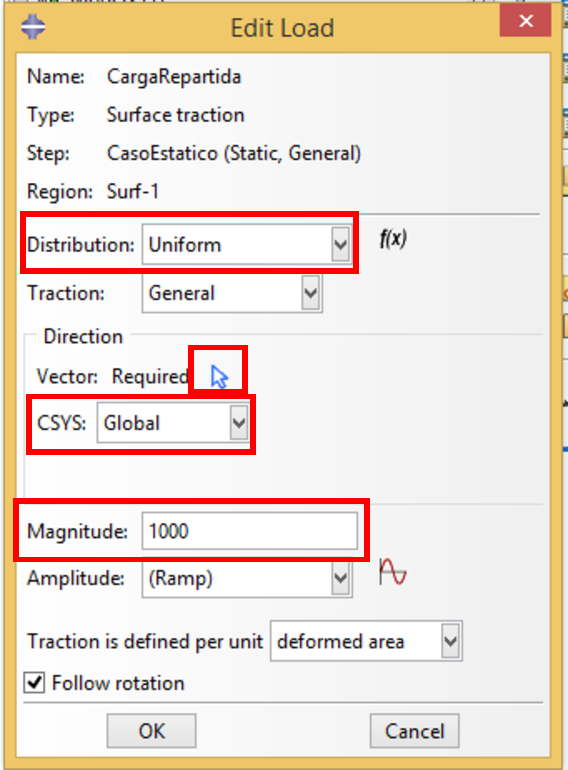
\includegraphics[width=\textwidth]{./body/images/imagen46.pdf}
\caption{Propiedades del vector tensión}
\label{figu46}
\end{subfigure}
\end{varwidth}\quad%\quad
\begin{varwidth}{0.60\linewidth}  % this is a must
\begin{subfigure}{0.95\textwidth}
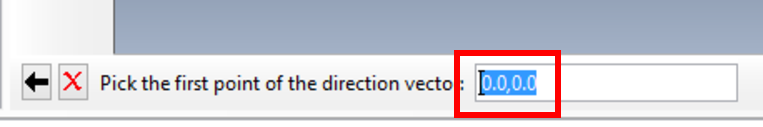
\includegraphics[width=\textwidth]{./body/images/imagen47.pdf}
\caption{Inicio vector auxiliar}
\label{figu47}
\end{subfigure}
\\
\begin{subfigure}{0.95\textwidth}

\includegraphics[width=\textwidth]{./body/images/imagen48.pdf}
\caption{Final vector auxiliar}
\label{figu48}
\end{subfigure}
\end{varwidth}
\caption{Definición carga repartida (II)} 
\end{figure}




\item Ahora nos aparece en el cuadro de diálogo anterior el vector
  normalizado (ver Fig.~\ref{figu49}) y, al aceptar la definición, nos
  aparece en la ventana de trabajo el esquema de distribución de
  cargas (ver Fig.~\ref{figu50}). Revisa en el \textbf{Model Tree} que
  se han añadido los nodos asociados a las condiciones de contorno.
  \begin{figure}[H]
    \centering
    \begin{subfigure}{0.30\textwidth}
      \includegraphics[width=\textwidth]{./body/images/imagen49.pdf}
      \caption{Propiedades del vector tensión}
      \label{figu49}
    \end{subfigure}%
    ~ %add desired spacing between images, e. g. ~, \quad, \qquad, \hfill etc.
    % (or a blank line to force the subfigure onto a new line)
    \begin{subfigure}{0.67\textwidth}
      \includegraphics[width=\textwidth]{./body/images/imagen50.pdf}
      \caption{Detalle carga aplicada }
      \label{figu50}
    \end{subfigure}%
    \caption{Definición carga repartida (III)}
  \end{figure}
\end{enumerate}
\newpage

\subsection{Módulo Mesh. Crear la malla.}
Para asignar una malla a una geometría le debemos informar a Abaqus
sobre:
\begin{enumerate}
\item la forma del elemento (si son triángulos o cuadrados en
  problemas bidimensionales y si son tetraedros o hexaedros en
  problemas tridimensionales).
\item tamaño del elemento (bien un tamaño global para la geometría o
  bien definir tamaños diferentes según regiones).
\item El tipo de elemento (nos lo explicarán en el resto del curso).
\end{enumerate}

Abaqus distingue qué tipo de malla puede realizar según la geometría
que tengamos (aunque el usuario puede dividir las \textit{parts}
manualmente para crear geometrías más regulares). Cada tipo de malla
posible en cada región la identifica con un color:
\begin{description}
\item[Verde] Se pueden generar mallas con métodos estructurados
\item[Amarillo] Se pueden generar mallas con el método de barrido
\item[Rosa] Se pueden generar mallas con el método libre
\item[Canela] Se pueden generar mallas con el método botton-up
\item[Naranja] No se pueden generar mallas y la geometría se tiene que
  dividir
\end{description}

En nuestro caso nos aparece que la geometría está de color azul. Esto
es porque hemos hecho una copia dependiente de la \textit{part} y es
ella la que tenemos que mallar (luego la malla se replica en la
copia). Activa el módulo \textbf{Mesh} y cambia a que el objeto a
mallar sea la \textit{part} tal como indica la Fig.~\ref{figu51} y
pasará a ponerse rosa.
\begin{figure}[H]
  \centering
  \includegraphics[width=0.95\textwidth]{./body/images/imagen51.pdf}
  \caption{Inicio módulo Mesh}
  \label{figu51}
\end{figure}

Para definir la malla sigue los siguientes pasos:
\begin{enumerate}
\item Primero definiremos la forma de los elementos. Pulsamos
  \textbf{Mesh/Controls} en barra superior de menús y nos aparece el
  cuadro de diálogo de la Fig.~\ref{figu52}. Indiquemos que queremos
  usar elementos \textbf{cuadriláteros}, que la técnica sea
  \textbf{Free} y que el algoritmo es \textbf{Advancing front}.
  \begin{figure}[H]
    \centering
    \includegraphics[width=0.50\textwidth]{./body/images/imagen52.pdf}
    \caption{Definición forma de los elementos}
    \label{figu52}
  \end{figure}
\item Definamos ahora el tamaño de los elementos. Pulsamos el icono
  \textbf{Seed part} (ver Fig.~\ref{figu53}) para asignar un tamaño
  global a los elementos de la geometría. Usemos un tamaño de 0.2 m
  tal como indica la Fig.~\ref{figu54} y pulsemos el botón
  \textbf{Aplicar}. Nos deberá aparecer una división de la frontera de
  nuestra geometría usando el tamaño que hemos indicado (ver
  Fig.~\ref{figu55}). Por último pulsa OK.

  \begin{figure}[H]
    \centering
    \begin{subfigure}{0.15\textwidth}
      \includegraphics[width=\textwidth]{./body/images/imagen53.pdf}
      \caption{Inicio comando \textbf{Seed part}}
      \label{figu53}
    \end{subfigure}%
    ~ %add desired spacing between images, e. g. ~, \quad, \qquad, \hfill etc.
    % (or a blank line to force the subfigure onto a new line)
    \begin{subfigure}{0.33\textwidth}
      \includegraphics[width=\textwidth]{./body/images/imagen54.pdf}
      \caption{Asignación global del tamaño de elemento}
      \label{figu54}
    \end{subfigure}%
    ~ %add desired spacing between images, e. g. ~, \quad, \qquad, \hfill etc.
    % (or a blank line to force the subfigure onto a new line)
    \begin{subfigure}{0.49\textwidth}
      \includegraphics[width=\textwidth]{./body/images/imagen55}
      \caption{Detalle división del contorno para la malla}
      \label{figu55}
    \end{subfigure}%
    \caption{Asignación tamaño global de la malla}
  \end{figure}
\item Definamos ahora el tipo de elemento pulsando el icono
  \textbf{Assign Element Type} (ver Fig.~\ref{figu56}). Nos pedirá que
  seleccionemos la \textit{Part} a la que le asignaremos el tipo de
  elemento.  Al seleccionarle nos deberá cambiar de color tal como
  indica la Fig.~\ref{figu57}. Por último nos aparece un cuadro de
  diálogo con los tipos de elementos disponibles. Tal como muestra la
  Fig.~\ref{figu58} seleccionemos \textbf{Standard},
  \textbf{Quadratic}, \textbf{Plane Stress} y \textbf{Reduced
    Integration} (ya irás aprendiendo en el resto del curso qué
  significan estos nombres).
  \begin{figure}[H]
    \centering
    \begin{subfigure}{0.15\textwidth}
      \includegraphics[width=\textwidth]{./body/images/imagen56.pdf}
      \caption{Inicio comando \textbf{Assign Element Type}}
      \label{figu56}
    \end{subfigure}%
    ~ %add desired spacing between images, e. g. ~, \quad, \qquad, \hfill etc.
    % (or a blank line to force the subfigure onto a new line)
    \begin{subfigure}{0.33\textwidth}
      \includegraphics[width=\textwidth]{./body/images/imagen57}
      \caption{Selección de la part}
      \label{figu57}
    \end{subfigure}%
    ~ %add desired spacing between images, e. g. ~, \quad, \qquad, \hfill etc.
    % (or a blank line to force the subfigure onto a new line)
    \begin{subfigure}{0.49\textwidth}
      \includegraphics[width=\textwidth]{./body/images/imagen58.pdf}
      \caption{Características del tipo de elemento}
      \label{figu58}
    \end{subfigure}%
    \caption{Definición tipo de elemento}
  \end{figure}
\item Una vez definida todos los parámetros de la malla solo falta
  generarla. Pulsamos el icono \textbf{Mesh Part} (ver
  Fig.~\ref{figu59}) y debes obtener la malla que muestra la
  Fig.~\ref{figu60}.
  \begin{figure}[H]
    \centering
    \begin{subfigure}{0.35\textwidth}
      \includegraphics[width=\textwidth]{./body/images/imagen59.pdf}
      \caption{Inicio Comando \textbf{Mesh Part} }
      \label{figu59}
    \end{subfigure}%
    ~ %add desired spacing between images, e. g. ~, \quad, \qquad, \hfill etc.
    % (or a blank line to force the subfigure onto a new line)
    \begin{subfigure}{0.60\textwidth}
      \includegraphics[width=\textwidth]{./body/images/imagen60}
      \caption{Malla final}
      \label{figu60}
    \end{subfigure}%
    \caption{Generación de la malla}
  \end{figure}
\end{enumerate}
\newpage
\subsection{Módulo Job. Crear el trabajo y lanzar el análisis.}

En este momento debemos tener un modelo de elementos finitos completo
que puede ser ejecutado. Antes de correr la simulación en Abaqus,
necesitamos crear un trabajo (\textbf{job}) y lanzarlo para que Abaqus
entienda que hay un modelo de elementos finitos listo para ser
simulado.

Para crear y lanzar un trabajo (\textbf{job}) sigue los siguientes
pasos:
\begin{enumerate}
\item Activa el módulo \textbf{job} y pulsa el icono \textbf{Create
    job} (ver Fig.~\ref{figu61}). Asígnale el nombre \textit{Caso01} e
  indica que los datos para el análisis debe tomarlos del Modelo que
  hemos creado y no de un fichero de entrada de datos \texttt{.inp}
  (ver Fig.~\ref{figu62}). Te aparecerá un cuadro de diálogo para
  definir el análisis (ver Fig.~\ref{figu63}). Incluye una descripción
  y deja el resto de parámetros por defecto.
  \begin{figure}[H]
    \centering
    \begin{subfigure}{0.15\textwidth}
      \includegraphics[width=\textwidth]{./body/images/imagen61.pdf}
      \caption{Comando \textbf{Create job}}
      \label{figu61}
    \end{subfigure}%
    ~ %add desired spacing between images, e. g. ~, \quad, \qquad, \hfill etc.
    % (or a blank line to force the subfigure onto a new line)
    \begin{subfigure}{0.33\textwidth}
      \includegraphics[width=\textwidth]{./body/images/imagen62.pdf}
      \caption{Inicio caso de análisis}
      \label{figu62}
    \end{subfigure}%
    ~ %add desired spacing between images, e. g. ~, \quad, \qquad, \hfill etc.
    % (or a blank line to force the subfigure onto a new line)
    \begin{subfigure}{0.49\textwidth}
      \includegraphics[width=\textwidth]{./body/images/imagen63.pdf}
      \caption{Parámetros del análisis}
      \label{figu63}
    \end{subfigure}%
    \caption{Creación de un nuevo análisis (\textbf{job})}
  \end{figure}
\item Vemos que se ha creado en el \textbf{Model Tree} un nuevo job
  (debajo de \textit{Analysis}). Para lanzarlo activemos el gestor de
  trabajos pulsando con el botón derecho del ratón encima de
  \textbf{Jobs} y seleccionando \textbf{Manager} (ver
  Fig.~\ref{figu65}). Nos aparece un cuadro de diálogo (ver
  Fig.~\ref{figu66}) que nos permite gestionar todos los análisis que
  tengamos (en este caso sólo tenemos uno, \textit{Caso01}). Pulsa
  \textbf{Write Input} para escribir en disco el fichero
  \texttt{caso01.inp} por si lo quisiéramos utilizar más adelante.
  \begin{figure}[H]
    \centering
    \begin{subfigure}{0.33\textwidth}
      \includegraphics[width=\textwidth]{./body/images/imagen65.pdf}
      \caption{Inicio gestor de los casos de análisis}
      \label{figu65}
    \end{subfigure}%
    ~ %add desired spacing between images, e. g. ~, \quad, \qquad, \hfill etc.
    % (or a blank line to force the subfigure onto a new line)
    \begin{subfigure}{0.49\textwidth}
      \includegraphics[width=\textwidth]{./body/images/imagen66.pdf}
      \caption{Gestor de casos de análisis}
      \label{figu66}
    \end{subfigure}%
    \caption{Ejecutar caso de análisis (I)}
  \end{figure}
\item Finalmente podemos lanzar el análisis. Podemos lanzarlo
  directamente pulsando \textbf{Submit} o podemos primero revisar que
  todo está bien pulsando \textbf{Data Check} y luego
  \textbf{Continue}. De cualquiera de las dos formas, si todo va bien,
  debes generar la parte inferior de la pantalla el mensaje de la
  Fig.~\ref{figu67} y en el gestor de casos el estatus del trabajo
  debe haber cambiado a \textbf{Completed} (ver Fig.~\ref{figu68}).
  \begin{figure}[H]
    \centering
    \begin{subfigure}{0.33\textwidth}
      \includegraphics[width=\textwidth]{./body/images/imagen67}
      \caption{Mensaje tras la ejecución del cálculo numérico}
      \label{figu67}
    \end{subfigure}%
    ~ %add desired spacing between images, e. g. ~, \quad, \qquad, \hfill etc.
    % (or a blank line to force the subfigure onto a new line)
    \begin{subfigure}{0.49\textwidth}
      \includegraphics[width=\textwidth]{./body/images/imagen68.pdf}
      \caption{Gestor de casos de análisis}
      \label{figu68}
    \end{subfigure}%
    \caption{Ejecutar caso de análisis (II)}
  \end{figure}
\end{enumerate}
\newpage
\subsection{Módulo Visualization. Realizar el post-proceso.}

Antes de empezar la visualización recordemos qué tipos de variables
tenemos y dónde se calculan. Primero veamos los tipos de variables y
la información que da Abaqus sobre ellas:
\begin{itemize}
\item Variables escalares (Temperatura $\theta$): 1 componente
\item Variables vectoriales (Desplazamiento $\mathbf{u}$): 3
  componentes + su módulo
\item Variables tensoriales orden 2 (tensiones $\bm{\sigma}$): 6
  componentes + valores invariantes respecto al sistema coordenado
  (von Mises, valores principales, tensión hidrostática)
\end{itemize}

Las variables desplazamiento y temperatura se calculan en los nodos de
la malla. Las variables flujo de calor, tensión y deformación se
calculan en los puntos de integración de los elementos. Estos valores
son luego extrapolados a los nodos de los elementos y posteriormente
suavizados en los nodos de la malla (ponderando la contribución de
todos los elementos que comparten un mismo nodo) tal como esquematiza
la Fig.~\ref{figu69}.
\begin{figure}[H]
  \centering
  \includegraphics[width=0.99\textwidth]{./body/images/imagen69}
  \caption{Proceso de suavizado de las variables definidas en puntos
    de integración}
  \label{figu69}
\end{figure}

Para activar el postproceso del análisis que acabamos de realizar
pulsa con el botón derecho del ratón sobre el job completado
\textit{Caso01} y selecciona \textbf{Results} tal como indica la
Fig.~\ref{figu70}.
\begin{figure}[H]
  \centering
  \includegraphics[width=0.29\textwidth]{./body/images/imagen70.pdf}
  \caption{Inicio postproceso de resultados}
  \label{figu70}
\end{figure}

A continuación vamos a describir alguna de las acciones más comunes
que se realizan en el postproceso de resultados:
\begin{enumerate}
\item \textbf{Dibujar la deformada de la malla}. ~

  Con el módulo \textbf{Visualization} activado pulsa el icono
  \textbf{Plot Deformed Shace} (ver Fig.~\ref{figu71}) para obtener la
  deformada. Obtendrás la deformada que se muestra en la
  Fig.~\ref{figu72} en la que los desplazamientos se han multiplicado
  por un factor de escala de 1.633e4.
  \begin{figure}[H]
    \centering
    \begin{subfigure}{0.25\textwidth}
      \includegraphics[width=\textwidth]{./body/images/imagen71.pdf}
      \caption{Comando \textbf{Plot Deformed Shape}}
      \label{figu71}
    \end{subfigure}%
    ~ %add desired spacing between images, e. g. ~, \quad, \qquad, \hfill etc.
    % (or a blank line to force the subfigure onto a new line)
    \begin{subfigure}{0.59\textwidth}
      \includegraphics[width=\textwidth]{./body/images/imagen72}
      \caption{Imagen de la deformada (factor de escala automático)}
      \label{figu72}
    \end{subfigure}%
    \caption{Representación de la deformada (I)}
  \end{figure}

  Para usar un factor de escala no automático pulsa el icono
  \textbf{Common Options} (ver Fig.~\ref{figu75}) Te aparecerá el
  cuadro de diálogo de la Fig.~\ref{figu73} en el que debes cambiar el
  \textbf{Deformation Scale Factor} a \textbf{Uniform} e indicar un
  valor de 10000. Al final obtendrás la deformada que muestra la
  Fig.~\ref{figu74}.

  \begin{figure}[H]
    \centering
    \begin{subfigure}{0.19\textwidth}
      \includegraphics[width=\textwidth]{./body/images/imagen75.pdf}
      \caption{Comando \textbf{Common Options}}
      \label{figu75}
    \end{subfigure}%
    ~ %add desired spacing between images, e. g. ~, \quad, \qquad, \hfill etc.
    % (or a blank line to force the subfigure onto a new line)
    \begin{subfigure}{0.30\textwidth}
      \includegraphics[width=\textwidth]{./body/images/imagen73.pdf}
      \caption{Opciones del postproceso}
      \label{figu73}
    \end{subfigure}%
    ~ %add desired spacing between images, e. g. ~, \quad, \qquad, \hfill etc.
    % (or a blank line to force the subfigure onto a new line)
    \begin{subfigure}{0.49\textwidth}
      \includegraphics[width=\textwidth]{./body/images/imagen74}
      \caption{Imagen de la deformada (factor de escala 10000)}
      \label{figu74}
    \end{subfigure}%
    \caption{Representación de la deformada (II)}
  \end{figure}
\item \textbf{Obtener la distribución de un escalar (una variable
    escalar o una componente de una variable vectorial o tensorial) en
    la geometría} ~

  Pulsa el icono \textbf{Plot Contours on Deformed Shape} o
  \textbf{Plot Contours on Undeformed Shape} (ver
  Fig.~\ref{figu76}). Nos aparecerá (bien en la geometría deformada o
  bien sin deformar) la distribución de un campo de la solución tal
  como muestra la Fig.~\ref{figu77} (en este caso es la componente
  $\sigma_{xx}$ del tensor de tensiones). Para cambiar qué variable
  deseas mostrar, selecciona la variable que desees dibujar en los
  menús desplegables en la barra de herramientas superior (ver
  Fig.~\ref{figu78}).
  \begin{figure}[H]
    \centering
    \begin{subfigure}{0.19\textwidth}
      \includegraphics[width=\textwidth]{./body/images/imagen76.pdf}
      \caption{Comando \textbf{Plot Contours on Deformed Shape}}
      \label{figu76}
    \end{subfigure}%
    ~ %add desired spacing between images, e. g. ~, \quad, \qquad, \hfill etc.
    % (or a blank line to force the subfigure onto a new line)
    \begin{subfigure}{0.44\textwidth}
      \includegraphics[width=\textwidth]{./body/images/imagen77}
      \caption{Deformada con el campo de $\sigma_{xx}$}
      \label{figu77}
    \end{subfigure}%
    ~ %add desired spacing between images, e. g. ~, \quad, \qquad, \hfill etc.
    % (or a blank line to force the subfigure onto a new line)
    \begin{subfigure}{0.35\textwidth}
      \includegraphics[width=\textwidth]{./body/images/imagen78.pdf}
      \caption{Selección de la componente de un resultado}
      \label{figu78}
    \end{subfigure}%
    \caption{Distribución de un campo escalar en la geometría (I)}
  \end{figure}

  Podemos modificar cómo se presentan estos campos de la
  solución. Pulsa el icono \textbf{Contour Options} (ver
  Fig.~\ref{figu79}) y en cuadro de diálogo resultante selecciona el
  tipo de contorno \textbf{Line} y los intervalos del contorno
  \textbf{Discrete} igual a 20 tal como muestra la
  Fig.~\ref{figu80}. Deberás obtener (para la variable que estés
  pintando) una distribución similar a la que muestra la
  Fig.~\ref{figu81}. Finalmente puedes guardar un archivo gráfico con
  los datos de la pantalla de trabajo pulsando \textbf{File/Print}
  para guardar un archivo \texttt{.pdf}, o pulsar \texttt{CTRL+C} para
  guardar la imagen en tu cripboard.

  \begin{figure}[H]
    \centering
    \begin{subfigure}{0.19\textwidth}
      \includegraphics[width=\textwidth]{./body/images/imagen79.pdf}
      \caption{Comando \textbf{Contour Options}}
      \label{figu79}
    \end{subfigure}%
    ~ %add desired spacing between images, e. g. ~, \quad, \qquad, \hfill etc.
    % (or a blank line to force the subfigure onto a new line)
    \begin{subfigure}{0.35\textwidth}
      \includegraphics[width=\textwidth]{./body/images/imagen80.pdf}
      \caption{Propiedades del \textbf{Contour Plot}}
      \label{figu80}
    \end{subfigure}%
    ~ %add desired spacing between images, e. g. ~, \quad, \qquad, \hfill etc.
    % (or a blank line to force the subfigure onto a new line)
    \begin{subfigure}{0.44\textwidth}
      \includegraphics[width=\textwidth]{./body/images/imagen81}
      \caption{Representación de un campo usando líneas de isovalores}
      \label{figu81}
    \end{subfigure}%
    \caption{Distribución de un campo escalar en la geometría (II)}
  \end{figure}

\item \textbf{Dibujar vectores o componentes principales de tensores
    en la geometría} ~

  Pulsa el icono \textbf{Plot Symbols on Deformed Shape} o
  \textbf{Plot Symbols on Undeformed Shape} (ver
  Fig.~\ref{figu82}). Te aparecerá una distribución de vectores tal
  como muestra la Fig.~\ref{figu83} (en este caso es la distribución
  de las componentes principales del tensor de tensiones en los puntos
  de integración de los elementos.

  \begin{figure}[H]
    \centering
    \begin{subfigure}{0.29\textwidth}
      \includegraphics[width=\textwidth]{./body/images/imagen82.pdf}
      \caption{Comando \textbf{Plot Symbols on Deformed Shape}}
      \label{figu82}
    \end{subfigure}%
    ~ %add desired spacing between images, e. g. ~, \quad, \qquad, \hfill etc.
    % (or a blank line to force the subfigure onto a new line)
    \begin{subfigure}{0.55\textwidth}
      \includegraphics[width=\textwidth]{./body/images/imagen83}
      \caption{Representación usando vectores}
      \label{figu83}
    \end{subfigure}%
    \caption{Distribución mediante vectores de una magnitud
      vectorial/tensorial (I)}
  \end{figure}

  Podemos modificar el formato de los vectores. En nuestro caso sería
  útil reducir un poco el tamaño para que se puedan ver mejor. Para
  hacerlo pulsa el icono \textbf{Symbol Options} (ver
  Fig.~\ref{figu84}) y en el siguiente cuadro de texto (ver
  Fig.~\ref{figu85}) cambia el tamaño a 2. Deberías obtener una
  distribución similar a la que muestra la Fig.~\ref{figu86}.

  \begin{figure}[H]
    \centering
    \begin{subfigure}{0.19\textwidth}
      \includegraphics[width=\textwidth]{./body/images/imagen84}
      \caption{Comando \textbf{Symbol Options}}
      \label{figu84}
    \end{subfigure}%
    ~ %add desired spacing between images, e. g. ~, \quad, \qquad, \hfill etc.
    % (or a blank line to force the subfigure onto a new line)
    \begin{subfigure}{0.35\textwidth}
      \includegraphics[width=\textwidth]{./body/images/imagen85}
      \caption{Opciones representación mediante vectores}
      \label{figu85}
    \end{subfigure}%
    ~ %add desired spacing between images, e. g. ~, \quad, \qquad, \hfill etc.
    % (or a blank line to force the subfigure onto a new line)
    \begin{subfigure}{0.44\textwidth}
      \includegraphics[width=\textwidth]{./body/images/imagen86}
      \caption{Representación usando vectores}
      \label{figu86}
    \end{subfigure}%
    \caption{Distribución mediante vectores de una magnitud
      vectorial/tensorial (II)}
  \end{figure}

\item \textbf{Obtener valores en nodos o en elementos}

  Hay veces que nos interesa saber valores de la solución en elementos
  o nodos específicos. Vamos a obtener primero la solución en
  elementos. Para hacerlo, primero debemos activar el \textbf{Plot
    Contour} con el campo que queramos conocer. Dibuja, como en la
  Fig.~\ref{figu87}, el campo de la componente $\sigma_{xx}$ del
  tensor de tensiones.  Después pulsa \textbf{tools/Query} (ver
  Fig.~\ref{figu88}) y selecciona \textbf{Probe values} (ver
  Fig.~\ref{figu89})

 \begin{figure}[H]
   \centering
   \begin{subfigure}{0.35\textwidth}
     \includegraphics[width=\textwidth]{./body/images/imagen87.pdf}
     \caption{Representación de un \textbf{Contour Plot}}
     \label{figu87}
   \end{subfigure}%
   ~ %add desired spacing between images, e. g. ~, \quad, \qquad, \hfill etc.
   % (or a blank line to force the subfigure onto a new line)
   \begin{subfigure}{0.29\textwidth}
     \includegraphics[width=\textwidth]{./body/images/imagen88.pdf}
     \caption{Comando \textbf{Tools/Query\ldots}}
     \label{figu88}
   \end{subfigure}%
   ~ %add desired spacing between images, e. g. ~, \quad, \qquad, \hfill etc.
   % (or a blank line to force the subfigure onto a new line)
   \begin{subfigure}{0.32\textwidth}
     \includegraphics[width=\textwidth]{./body/images/imagen89.pdf}
     \caption{Información que podemos obtener del modelo}
     \label{figu89}
   \end{subfigure}%
   \caption{Obtención valores en elementos (I)}
 \end{figure}

 Nos aparece un cuadro de diálogo en el que le vamos a indicar que
 queremos extraer valores de los \textbf{Elements}, que del campo
 seleccionado en el \textbf{Plot Contours} queremos \textbf{All
   Diections} y que queremos los valores en los \textbf{Integration
   Points} tal como indica la Fig.~\ref{figu90}. Seleccionamos uno a
 uno los elementos que están en contacto con el borde izquierdo de la
 ménsula (ver Fig.~\ref{figu91})

 \begin{figure}[H]
   \centering
   \begin{subfigure}{0.45\textwidth}
     \includegraphics[width=\textwidth]{./body/images/imagen90.pdf}
     \caption{Definición lugares donde se extrae la información}
     \label{figu90}
   \end{subfigure}%
   ~ %add desired spacing between images, e. g. ~, \quad, \qquad, \hfill etc.
   % (or a blank line to force the subfigure onto a new line)
   \begin{subfigure}{0.49\textwidth}
     \includegraphics[width=\textwidth]{./body/images/imagen91.pdf}
     \caption{Selección de los elementos}
     \label{figu91}
   \end{subfigure}%
   \caption{Obtención valores en elementos (II)}
 \end{figure}

 Una vez seleccionado los elementos pulsamos \textbf{Write to File}
 (ver Fig.~\ref{figu92}) y escribimos los resultados en un archivo
 \texttt{tensiones.rpt} (ver Fig.~\ref{figu93}). Si abrimos el fichero
 \texttt{tensiones.rpt} con un programa de textos ver cómo nos ha
 guardado los valores de las componentes del tensor de tensiones en
 los cuatro puntos de integración de cada uno de los elementos
 seleccionados (ver Fig.~\ref{figu94}).

 \begin{figure}[H]
   \centering
   \begin{subfigure}{0.32\textwidth}
     \includegraphics[width=\textwidth]{./body/images/imagen92.pdf}
     \caption{Elementos seleccionados}
     \label{figu92}
   \end{subfigure}%
   ~ %add desired spacing between images, e. g. ~, \quad, \qquad, \hfill etc.
   % (or a blank line to force the subfigure onto a new line)
   \begin{subfigure}{0.32\textwidth}
     \includegraphics[width=\textwidth]{./body/images/imagen93.pdf}
     \caption{Definición del archivo donde guardar los datos}
     \label{figu93}
   \end{subfigure}%
   ~ %add desired spacing between images, e. g. ~, \quad, \qquad, \hfill etc.
   % (or a blank line to force the subfigure onto a new line)
   \begin{subfigure}{0.35\textwidth}
     \includegraphics[width=\textwidth]{./body/images/imagen94}
     \caption{Información en modo texto de una variable en los
       elementos seleccionados}
     \label{figu94}
   \end{subfigure}%
   \caption{Obtención valores en elementos (III)}
 \end{figure}

 Vamos a obtener ahora la solución en nodos. Igual que antes activemos
 el \textbf{Plot Contour} con el campo que queramos conocer. Dibuja
 ahora, como en la Fig.~\ref{figu95}, el campo de la componente
 $R_{x}$ de las fuerzas de reacción. Recuerda que para activar el
 cuadro de diálogo \textbf{Probe Values} hay que pulsar
 \textbf{tools/Query} (ver Fig.~\ref{figu88}) y seleccionar
 \textbf{Probe values} (ver Fig.~\ref{figu89}). Indica que queremos
 obtener la solución en los \textbf{Nodes} y que queremos todas las
 componentes. Finalmente selecciona todos los nodos del borde
 izquierdo (ver Fig.~\ref{figu96}). Una vez seleccionados pulsa
 \textbf{Write to File} y guarda los datos en un fichero llamado
 \textbf{Reacciones}. Abre finalmente el fichero y comprueba que se
 han guardado los valores de las reacciones en los nodos seleccionados
 (ver Fig.~\ref{figu97}).

 \begin{figure}[H]
   \centering
   \begin{subfigure}{0.30\textwidth}
     \includegraphics[width=\textwidth]{./body/images/imagen95.pdf}
     \caption{Representación de un \textbf{Contour Plot}}
     \label{figu95}
   \end{subfigure}%
   ~ %add desired spacing between images, e. g. ~, \quad, \qquad, \hfill etc.
   % (or a blank line to force the subfigure onto a new line)
   \begin{subfigure}{0.30\textwidth}
     \includegraphics[width=\textwidth]{./body/images/imagen96.pdf}
     \caption{Selección de los nodos}
     \label{figu96}
   \end{subfigure}%
   ~ %add desired spacing between images, e. g. ~, \quad, \qquad, \hfill etc.
   % (or a blank line to force the subfigure onto a new line)
   \begin{subfigure}{0.39\textwidth}
     \includegraphics[width=\textwidth]{./body/images/imagen97}
     \caption{Información en modo texto de una variable en los nodos
       seleccionados}
     \label{figu97}
   \end{subfigure}%
   \caption{Obtención valores en nodos (I)}
 \end{figure}



 
\item \textbf{Obtener curvas} ~

  Finalmente vamos a dibujar la distribución de una variable de la
  solución siguiendo un camino en la geometría. Para eso primero
  tenemos que definir un camino (\textbf{Path}) dentro del modelo y
  luego obtener una curva X-Y en el que la abscisa X sea la distancia
  de un punto siguiendo el camino y la ordenada Y el valor en dicho
  punto de la variable.

  Dibuja de nuevo el campo de la componente $R_{x}$ de las fuerzas de
  reacción (ver Fig.~\ref{figu98}) y pulsa \textbf{Path/Create} (ver
  Fig.~\ref{figu99}). En el siguiente cuadro de diálogo asigna el
  nombre \textit{Path-empotramiento} al \textbf{path} e indica que es
  un \textbf{Node list} como indica la Fig.~\ref{figu100}.

 \begin{figure}[H]
   \centering
   \begin{subfigure}{0.30\textwidth}
     \includegraphics[width=\textwidth]{./body/images/imagen98}
     \caption{Representación de un \textbf{Contour Plot}}
     \label{figu98}
   \end{subfigure}%
   ~ %add desired spacing between images, e. g. ~, \quad, \qquad, \hfill etc.
   % (or a blank line to force the subfigure onto a new line)
   \begin{subfigure}{0.30\textwidth}
     \includegraphics[width=\textwidth]{./body/images/imagen99.pdf}
     \caption{Comando \textbf{Path/Create\ldots}}
     \label{figu99}
   \end{subfigure}%
   ~ %add desired spacing between images, e. g. ~, \quad, \qquad, \hfill etc.
   % (or a blank line to force the subfigure onto a new line)
   \begin{subfigure}{0.39\textwidth}
     \includegraphics[width=\textwidth]{./body/images/imagen100.pdf}
     \caption{Nombre y definición del tipo de \textbf{Path}}
     \label{figu100}
   \end{subfigure}%
   \caption{Definición de un \textbf{Path} (I)}
 \end{figure}

 En el siguiente cuadro de diálogo debemos empezar asignar los
 nodos. Selecciona \textbf{Add After} (aunque en este caso daría igual
 \textbf{Add Before} porque no tenemos una selección previa) como
 indica la Fig.~\ref{figu101}. Marca el punto inicial (extremo
 superior del empotramiento) y el punto final (extremo inferior del
 empotramiento) para definir el camino (ver
 Fig.~\ref{figu102}). Finalmente deberías obtener el cuadro de diálogo
 de la Fig.~\ref{figu103}.

 \begin{figure}[H]
   \centering
   \begin{subfigure}{0.30\textwidth}
     \includegraphics[width=\textwidth]{./body/images/imagen101.pdf}
     \caption{Definición nodos del path (I)}
     \label{figu101}
   \end{subfigure}%
   ~ %add desired spacing between images, e. g. ~, \quad, \qquad, \hfill etc.
   % (or a blank line to force the subfigure onto a new line)
   \begin{subfigure}{0.30\textwidth}
     \includegraphics[width=\textwidth]{./body/images/imagen102}
     \caption{Definición nodos del path (II)}
     \label{figu102}
   \end{subfigure}%
   ~ %add desired spacing between images, e. g. ~, \quad, \qquad, \hfill etc.
   % (or a blank line to force the subfigure onto a new line)
   \begin{subfigure}{0.39\textwidth}
     \includegraphics[width=\textwidth]{./body/images/imagen103.pdf}
     \caption{Definición nodos del path (III)}
     \label{figu103}
   \end{subfigure}%
   \caption{Definición de un \textbf{Path} (II)}
 \end{figure}

 Una vez definido el \textbf{path} podemos definir el gráfico
 X-Y. Pulsa \textbf{Tools/XY DAta/Create} tal como indica la
 Fig.~\ref{figu104} e indica que la fuente para las abscisas va a ser
 \textbf{Path} (ver Fig.~\ref{figu105}). En el siguiente cuadro de
 diálogo para definir el gráfico indica que el path es el que hemos
 creado \textit{Path-empotramiento}, que seguiremos la deformada
 (\textbf{Deformed}, que queremos que incluya las intersecciones y que
 el valor de la abscisa es la distancia verdadera siguiendo el camino
 (revisa la Fig.~\ref{figu106}). Para seleccionar la variable que
 queremos que nos dibuje pulsa \textbf{Field Output...} (ver
 Fig.~\ref{figu106}).

\begin{figure}[H]
  \centering
  \begin{subfigure}{0.30\textwidth}
    \includegraphics[width=\textwidth]{./body/images/imagen104.pdf}
    \caption{Comando \textbf{Tools/XY DAta/Create} }
    \label{figu104}
  \end{subfigure}%
  ~ %add desired spacing between images, e. g. ~, \quad, \qquad, \hfill etc.
  % (or a blank line to force the subfigure onto a new line)
  \begin{subfigure}{0.30\textwidth}
    \includegraphics[width=\textwidth]{./body/images/imagen105.pdf}
    \caption{Origen de los datos}
    \label{figu105}
  \end{subfigure}%
  ~ %add desired spacing between images, e. g. ~, \quad, \qquad, \hfill etc.
  % (or a blank line to force the subfigure onto a new line)
  \begin{subfigure}{0.39\textwidth}
    \includegraphics[width=\textwidth]{./body/images/imagen106.pdf}
    \caption{Cuadro de características del gráfico X-Y}
    \label{figu106}
  \end{subfigure}%
  \caption{Definición curva X-Y (I)}
\end{figure}

De las opciones que nos ofrece la siguiente ventana (ver
Fig.~\ref{figu107}) elegimos la componente \textbf{RF1} de las fuerzas
de reacción en los nodos (\textbf{RF}). De nuevo en el cuadro de
diálogo \textbf{XY Data from Path} pulsamos \textbf{Plot} y debemos
obtener la curva que muestra la Fig.~\ref{figu108}. Finalmente
pulsamos \textbf{Save as\ldots} y guardamos el gráfico con el nombre
\textit{XYData-Rx} (ver Fig.~\ref{figu109}).


\begin{figure}[H]
\centering
\begin{varwidth}{0.45\linewidth}  % this is a must
\begin{subfigure}{0.95\textwidth}
\includegraphics[width=\textwidth]{./body/images/imagen107.pdf}
\caption{Selección de la variable a dibujar}
\label{figu107}
\end{subfigure}
\end{varwidth}\quad%\quad
\begin{varwidth}{0.55\linewidth}  % this is a must
\begin{subfigure}{0.99\textwidth}
\includegraphics[width=\textwidth]{./body/images/imagen108}
\caption{Valores de Rx en el lado del empotramiento}
\label{figu108}
\end{subfigure}
\\
\begin{subfigure}{0.75\textwidth}
\includegraphics[width=\textwidth]{./body/images/imagen109.pdf}
\caption{Nombre del gráfico (se guarda sólo para la sesión)}
\label{figu109}
\end{subfigure}
\end{varwidth}
\caption{Definición curva X-Y (II)}
\end{figure}

% \begin{figure}[H]
%   \centering
%   \begin{subfigure}{0.30\textwidth}
%     \includegraphics[width=\textwidth]{./body/images/imagen107.pdf}
%     \caption{Selección de la variable a dibujar}
%     \label{figu107}
%   \end{subfigure}%
%   ~ %add desired spacing between images, e. g. ~, \quad, \qquad, \hfill etc.
%   % (or a blank line to force the subfigure onto a new line)
%   \begin{subfigure}{0.39\textwidth}
%     \includegraphics[width=\textwidth]{./body/images/imagen108}
%     \caption{Valores de Rx en el lado del empotramiento}
%     \label{figu108}
%   \end{subfigure}%
%   ~ %add desired spacing between images, e. g. ~, \quad, \qquad, \hfill etc.
%   % (or a blank line to force the subfigure onto a new line)
%   \begin{subfigure}{0.30\textwidth}
%     \includegraphics[width=\textwidth]{./body/images/imagen109.pdf}
%     \caption{Nombre del gráfico (se guarda sólo para la sesión)}
%     \label{figu109}
%   \end{subfigure}%
%   \caption{Definición curva X-Y (II)}
% \end{figure}

Finalmente buscamos guardar los datos de la curva que hemos creado en
un fichero de texto para poder usarla en otro programa. Selecciona
\textbf{Report/XY \ldots} (ver Fig.~\ref{figu110}) y, en la siguiente
ventana selecciona la gráfica que hemos creado \textit{XYData-Rx} en
la pestaña \textbf{XY Data} (ver Fig.~\ref{figu111}) y el nombre de
fichero \textbf{curvas.rpt} en la pestaña \textbf{Setup} (ver
Fig.~\ref{figu112}). Si abres un fichero de texto deberías obtener
algo parecido a los datos de la Fig.~\ref{figu113}.


\begin{figure}[H]
  \centering
  \begin{subfigure}{0.30\textwidth}
    \includegraphics[width=\textwidth]{./body/images/imagen110.pdf}
    \caption{Comando \textbf{Report/XY \ldots}}
    \label{figu110}
  \end{subfigure}%
  ~ %add desired spacing between images, e. g. ~, \quad, \qquad, \hfill etc.
  % (or a blank line to force the subfigure onto a new line)
  \begin{subfigure}{0.50\textwidth}
    \includegraphics[width=\textwidth]{./body/images/imagen111.pdf}
    \caption{Escritura datos gráfico X-Y (I)}
    \label{figu111}
  \end{subfigure}%
  
 %add desired spacing between images, e. g. ~, \quad, \qquad, \hfill etc.
  % (or a blank line to force the subfigure onto a new line)
  \begin{subfigure}{0.50\textwidth}
    \includegraphics[width=\textwidth]{./body/images/imagen112.pdf}
    \caption{Escritura datos gráfico X-Y (II)}
    \label{figu112}
  \end{subfigure}%
  ~ %add desired spacing between images, e. g. ~, \quad, \qquad, \hfill etc.
  % (or a blank line to force the subfigure onto a new line)
  \begin{subfigure}{0.50\textwidth}
    \includegraphics[width=\textwidth]{./body/images/imagen113}
    \caption{Datos curva X-Y en formato texto}
    \label{figu113}
  \end{subfigure}%
  \caption{Definición curva X-Y (III)}
\end{figure}

\end{enumerate}

\hspace{20mm}\hrulefill$\star$\hrulefill\hspace{20mm}
